%%
%%  Copyright 2023 CEA*
%%  *Commissariat a l'Energie Atomique et aux Energies Alternatives (CEA)
%%
%%  SPDX-License-Identifier: Apache-2.0 WITH SHL-2.1
%%
%%  Licensed under the Solderpad Hardware License v 2.1 (the “License”); you
%%  may not use this file except in compliance with the License, or, at your
%%  option, the Apache License version 2.0. You may obtain a copy of the
%%  License at
%%
%%  https://solderpad.org/licenses/SHL-2.1/
%%
%%  Unless required by applicable law or agreed to in writing, any work
%%  distributed under the License is distributed on an “AS IS” BASIS, WITHOUT
%%  WARRANTIES OR CONDITIONS OF ANY KIND, either express or implied. See the
%%  License for the specific language governing permissions and limitations
%%  under the License.
%%
%%  Author(s):          Cesar Fuguet
%%  Date:               February, 2023
%%  Description:        Specification document of the HPDcache hardware IP
%%
\documentclass[10pt,titlepage,twoside]{book}
\newcommand{\doctitle}{High-Performance, Multi-Requester, Out-of-Order, L1 Dcache (HPDcache)}
\newcommand{\docauthor}{César Fuguet}
\newcommand{\docdate}{February, 2023}

%%
%%  Copyright 2023 CEA*
%%  *Commissariat a l'Energie Atomique et aux Energies Alternatives (CEA)
%%
%%  SPDX-License-Identifier: Apache-2.0 WITH SHL-2.1
%%
%%  Licensed under the Solderpad Hardware License v 2.1 (the “License”); you
%%  may not use this file except in compliance with the License, or, at your
%%  option, the Apache License version 2.0. You may obtain a copy of the
%%  License at
%%
%%  https://solderpad.org/licenses/SHL-2.1/
%%
%%  Unless required by applicable law or agreed to in writing, any work
%%  distributed under the License is distributed on an “AS IS” BASIS, WITHOUT
%%  WARRANTIES OR CONDITIONS OF ANY KIND, either express or implied. See the
%%  License for the specific language governing permissions and limitations
%%  under the License.
%%
%%  Author(s):          Cesar Fuguet
%%  Date:               February, 2023
%%  Description:        Specification document of the HPDcache hardware IP
%%

%%%
%%  Font packages
%%%
\usepackage[T1]{fontenc}
\usepackage[utf8]{inputenc}
\usepackage{fourier}

\usepackage{amsmath}
\usepackage{amsthm}

%\usepackage{lmodern}
\usepackage{xcolor}

\definecolor{lightgray}{gray}{0.8}

% use Helvetica Adobe sans serif fonts
\renewcommand{\sfdefault}{phv}

%%%
%%  Language packages
%%%
\usepackage{csquotes}
\usepackage[english]{babel}

%%%
%%  Page margins configuration
%%%
\usepackage{geometry}
\geometry{top=3cm, bottom=3cm}

%%%
%%  Figures' configuration packages and command
%%%
\usepackage{ifpdf}

\ifpdf
\usepackage[pdftex]{graphicx}
\DeclareGraphicsExtensions{.jpg,.png,.pdf}
\else
\usepackage[dvips]{graphicx}
\DeclareGraphicsExtensions{{.eps}}
\fi

\usepackage[font=footnotesize,position=top,skip=0pt]{caption}
\usepackage[font=footnotesize,position=top,skip=0pt]{subcaption}

%%%
%%  Tables' configuration packages
%%%
\usepackage{booktabs}
\usepackage{tabularx}
\usepackage{multirow}

\newcolumntype{L}[1]{>{\hsize=#1\hsize\raggedright\arraybackslash}X}%
\newcolumntype{C}[1]{>{\hsize=#1\hsize\centering\arraybackslash}X}%

%%%
%%  Misc configuration
%%%
\usepackage{minitoc}
\usepackage{emptypage} % prevent headings in empty pages
\usepackage{xspace}
\usepackage{enumitem}
\usepackage[printonlyused]{acronym}
\usepackage{tikz}
\newcommand*\circled[1]{\tikz[baseline=(char.base)]{%
    \node[shape=circle,draw=black,inner sep=1pt] (char){\textsf{\bfseries #1}};%
  }%
}
\usetikzlibrary{shapes,arrows,chains}

% Color boxing
\usepackage[many]{tcolorbox}

%%%
%%  Math environments
%%%
\theoremstyle{plain}
\newtheorem{property}{Property}[section]
\newtheorem{lemma}{Lemma}[property]

\theoremstyle{definition}
\newtheorem{definition}{Definition}[section]

\newcommand{\eqvar}[1]{$\mathit{#1}$}
\renewcommand\qedsymbol{$\blacksquare$}

%%%
%%  Table of Contents (TOC), and chapters and section titles format
%%%
\usepackage{titletoc}
\usepackage{titlesec}

%%%
%%  To Do notes
%%%
\usepackage[%
  colorinlistoftodos,
  prependcaption
]{todonotes}

\ifdefined\isdraft
  \newcommand{\TodoSide}[1]{\todo[color=red!20]{\textbf{To do}: #1}}
  \newcommand{\NoteSide}[1]{\todo[color=green!20]{\textbf{Note}: #1}}
  \newcommand{\Todo}[1]{\todo[inline, color=red!20]{\textbf{To do}: #1}}
  \newcommand{\Note}[1]{\todo[inline, color=green!20]{\textbf{Note}: #1}}
\else
  \newcommand{\TodoSide}[1]{}
  \newcommand{\NoteSide}[1]{}
  \newcommand{\Todo}[1]{}
  \newcommand{\Note}[1]{}
\fi


% maximum depth of the table of contents (2: subsection)

\setcounter{tocdepth}{2}

% format for general table of contents
\titlecontents{chapter}%
[1.5em]%
{\addvspace{1em plus 0pt minus 0pt}\bfseries}%
{\contentslabel{1.3em}}%
{\hspace{-1.3em}}%
{\hfill\contentspage}%
[\addvspace{0pt}]

\titlecontents{section}%
[3.8em]%
{\addvspace{.4em plus 0pt minus 0pt}\bfseries}%
{\contentslabel{2.3em}}%
{}%
{\titlerule*[0.75em]{\normalfont.}\contentspage}

\titlecontents{subsection}%
[7.0em]%
{\addvspace{.2em plus 0pt minus 0pt}}%
{\contentslabel{3.2em}}%
{}%
{\titlerule*[.75em]{.}\contentspage}

% format for partial table of contents (at each chapter)

\titlecontents{psection}%
[2.3em]%
{\addvspace{.4em plus 0pt minus 0pt}\bfseries}%
{\contentslabel{2.3em}}%
{}%
{\titlerule*[.75em]{\normalfont.}\contentspage}

\titlecontents{psubsection}%
[5.5em]%
{\addvspace{.2em plus 0pt minus 0pt}}%
{\contentslabel{3.2em}}%
{}%
{\titlerule*[.75em]{.}\contentspage}

\titlecontents{figure}%
[3.8em]%
{\addvspace{.4em plus 0pt minus 0pt}\normalfont}%
{\contentslabel{2.3em}}%
{}%
{\titlerule*[0.75em]{\normalfont.}\contentspage}

\titlecontents{table}%
[3.8em]%
{\addvspace{.4em plus 0pt minus 0pt}\normalfont}%
{\contentslabel{2.3em}}%
{}%
{\titlerule*[0.75em]{\normalfont.}\contentspage}

% insert this command at each chapter's beginning to add a partial TOC

\newcommand{\chaptertoc}{%
  \vspace*{1.25ex}%
  \vbox{\bfseries\Large Contents}%
  \vspace*{1ex}\titlerule%
  \normalfont\normalsize%
  \startcontents[sections]%
  \printcontents[sections]{p}{1}{}%
  \vspace*{1ex}\titlerule\vspace*{1ex}%
  \newpage}

\titleformat{\chapter}[display]{\bfseries\huge}%
{\chaptertitlename~\thechapter}{.75ex}%
{\titlerule[2pt]\vspace*{.75ex}\filright}%
[]%[\vspace*{.75ex}\titlerule]
\titlespacing*{\chapter}{0pt}{30pt}{20pt}[0pt]

\titleformat{\section}[hang]{\normalfont\Large\bfseries}{%
  \thesection}{1em}{}
\titlespacing*{\section}{0pt}{%
  3.5ex plus 1ex minus .2ex}{2.3ex plus .2ex}[0pt]

\titleformat{\subsection}[hang]{\normalfont\large\bfseries}{%
  \thesubsection}{1em}{}
\titlespacing*{\subsection}{0pt}{%
  3.25ex plus 1ex minus .2ex}{1.5ex plus .2ex}[0pt]

\titleformat{\subsubsection}[hang]{\normalfont\normalsize\bfseries}{%
  \thesubsubsection}{1em}{}
\titlespacing*{\subsubsection}{0pt}{%
  3.25ex plus 1ex minus .2ex}{1.5ex plus .2ex}[0pt]

\titleformat{\paragraph}[runin]{\normalfont\normalsize\bfseries}{%
  \theparagraph}{1em}{}[]
\titlespacing*{\paragraph}{0pt}{%
  3.25ex plus 1ex minus .2ex}{1em}

\titleformat{\subparagraph}[runin]{\normalfont\normalsize\bfseries}{%
  \thesubparagraph}{1em}{}[]
\titlespacing*{\subparagraph}{\parindent}{%
  3.25ex plus 1ex minus .2ex}{1em}

%%%
%%  Header / footer configuration
%%%
\usepackage{fancyhdr}

\fancypagestyle{fancystyle}{%
  \fancyhf{}% clear header and footer fields
  \fancyhead[RO,LE]{\footnotesize\sffamily\nouppercase{\rightmark}}%
  \fancyhead[RE,LO]{\footnotesize\sffamily\mbox{}Version~\docversion}%
  \fancyfoot[LO,RE]{\footnotesize\sffamily\mbox{}\docauthor}%
  \fancyfoot[CE,CO]{\footnotesize\sffamily\mbox{}Copyright~\textcopyright~2023~Commissariat à l'Energie Atomique et aux Energies Alternatives (CEA)}%
  \fancyfoot[RO,LE]{\footnotesize\sffamily\mbox{}\thepage}%
  \renewcommand{\headrulewidth}{.6pt}%
  \renewcommand{\footrulewidth}{.6pt}%
}

\fancypagestyle{plain}{%
  \fancyhf{}% clear header and footer fields
  \fancyfoot[C]{\normalfont\sffamily\thepage}%
  \renewcommand{\headrulewidth}{0pt}%
  \renewcommand{\footrulewidth}{0pt}%
}

\renewcommand{\sectionmark}{\markright}

\addtolength{\headheight}{\baselineskip}

%%%
%%  Bibliography configuration
%%%
\usepackage[
    backend=biber,
    bibencoding=utf8,
    citestyle=ieee,
    style=ieee
]{biblatex}

%%%
%%  Hyperref package (must be declared at last to avoid conflicts)
%%%
\usepackage[pdfusetitle]{hyperref}
\usepackage{url}
\hypersetup{%
colorlinks,%
linkcolor=blue%
}

%%  Plot drawing package
\usepackage{pgfplots}

%%  Programming code formatting
\usepackage{listings}

%%  Algorithm formatting
\usepackage{algorithm}
\usepackage{algorithmic}

%%  Formatting of network protocol specification
\usepackage{bytefield}


%%%
%%  Definition of command aliases
%%%
%%%
%%  Add vertical space between paragraphs and remove indentation
%%%
\usepackage{parskip}

% keep the parskip for theorems (AMS packages).
\makeatletter
\def\thm@space@setup{%
  \thm@preskip=\parskip \thm@postskip=0pt
}
\makeatother

%%%
%%  Label and reference commands
%%%
\newcommand{\figfont}[1]{\textsf{\bfseries #1}}

\newcommand{\figlabel}[1]{\label{fig:#1}}
\newcommand{\Figref}[1]{\hyperref[fig:#1]{\mbox{Figure~\ref{fig:#1}}}}
\newcommand{\figref}[1]{\hyperref[fig:#1]{\mbox{figure~\ref{fig:#1}}}}
\newcommand{\fighypref}[2]{\hyperref[fig:#1]{#2}}
\newcommand{\chalabel}[1]{\label{cha:#1}}
\newcommand{\Charef}[1]{\hyperref[cha:#1]{\mbox{Chapter~\ref{cha:#1}}}}
\newcommand{\charef}[1]{\hyperref[cha:#1]{\mbox{chapter~\ref{cha:#1}}}}
\newcommand{\chafullref}[1]{Chapter~\ref{cha:#1}-\nameref{cha:#1}}
\newcommand{\chahypref}[2]{\hyperref[cha:#1]{#2}}
\newcommand{\seclabel}[1]{\label{sec:#1}}
\newcommand{\Secref}[1]{\hyperref[sec:#1]{\mbox{Section~\ref{sec:#1}}}}
\newcommand{\secref}[1]{\hyperref[sec:#1]{\mbox{section~\ref{sec:#1}}}}
\newcommand{\sechypref}[2]{\hyperref[sec:#1]{#2}}
\newcommand{\apxlabel}[1]{\label{apx:#1}}
\newcommand{\Apxref}[1]{\hyperref[apx:#1]{\mbox{Appendix~\ref{apx:#1}}}}
\newcommand{\apxref}[1]{\hyperref[apx:#1]{\mbox{appendix~\ref{apx:#1}}}}
\newcommand{\apxhypref}[2]{\hyperref[apx:#1]{#2}}
\newcommand{\tablabel}[1]{\label{tab:#1}}
\newcommand{\Tabref}[1]{\hyperref[tab:#1]{\mbox{Table~\ref{tab:#1}}}}
\newcommand{\tabref}[1]{\hyperref[tab:#1]{\mbox{table~\ref{tab:#1}}}}
\newcommand{\tabhypref}[2]{\hyperref[tab:#1]{#2}}
\newcommand{\alglabel}[1]{\label{alg:#1}}
\newcommand{\Algref}[1]{\hyperref[alg:#1]{\mbox{Algorithm~\ref{alg:#1}}}}
\newcommand{\algref}[1]{\hyperref[alg:#1]{\mbox{algorithm~\ref{alg:#1}}}}
\newcommand{\alghypref}[2]{\hyperref[alg:#1]{#2}}
\newcommand{\prplabel}[1]{\label{prp:#1}}
\newcommand{\prpref}[1]{\hyperref[prp:#1]{\mbox{Property~\ref{prp:#1}}}}
\newcommand{\lemlabel}[1]{\label{lem:#1}}
\newcommand{\lemref}[1]{\hyperref[lem:#1]{\mbox{Lemma~\ref{lem:#1}}}}
\newcommand{\deflabel}[1]{\label{def:#1}}
\newcommand{\defref}[1]{\hyperref[def:#1]{\mbox{Definition~\ref{def:#1}}}}



\title{\doctitle}
\author{\docauthor}

\addbibresource{hpdcache_spec.bib}

\begin{document}

\dominitoc

%
%  front-matter
%
\pagestyle{plain}

\begin{center}

  \mbox{}\vspace{3cm}

  {\huge\doctitle}\\

  \vfill

  {\normalsize%
  \begin{tabular}{p{.4\textwidth}l}
    \toprule
    Author:
    & \mbox{\docauthor} \\
    \midrule
    Release date:
    & \mbox{\docdate}
  \end{tabular}}

  \vfill

  This document version is~\docversion

  {\footnotesize\sffamily\mbox{}Copyright~\textcopyright~2023\\
  \mbox{\emph{Commissariat à l'Energie Atomique et aux Energies Alternatives (CEA)}}}
\end{center}

\clearpage

Contributors to all versions of this specification document:\\
Cesar Fuguet,
Adrian Evans,
Tanuj-Kumar Khandelwal,
Nicolas Perbost.

\clearpage
\tableofcontents
\listoftables
\listoffigures

\pagestyle{fancystyle}

%
%  acronyms
%
\clearpage
\chapter*{Table of Acronyms}

\begin{acronym}[YYYYYY]
\acro{CEA}{Commissariat à l'Energie Atomique et aux Energies Alternatives}
\acro{HPDcache}{High-Performance, Multi-Requester, Multi-Issue, Out-of-Order, L1 Dcache}
\acro{DMA}{Direct Memory Access}
\acro{GPP}{General Purpose Processor}
\acro{AMBA}{Advanced Microcontroller Bus Architecture}
\acro{AXI}{Advance eXtensible Interface}
\acro{NoC}{Network-on-Chip}
\acro{PoS}{Point-of-Serialization}
\acro{SLC}{System-Level Cache}
\acro{LSU}{Load-Store Unit}
\acro{MMU}{Memory Management Unit}
\acro{AMO}{Atomic Memory Operation}
\acro{CSR}{Configuration-and-Status Register}
\acro{CMO}{Cache Maintenance Operation}
\acro{HBM}{High-Bandwidth Memory}
\acro{MSHR}{Miss Status Holding Register}
\acro{RTAB}{Replay Table}
\acro{MCR}{Memory Consistency Rule}
\acro{RVWMO}{RISC-V Weak Memory Ordering}
\acro{WBUF}{Write Buffer}
\acro{ISA}{Instruction Set Architecture}
\acro{ASIC}{Application Specific Integrated Circuit}
\acro{FPGA}{Field-Programmable Gate Array}
\acro{SRAM}{Static Random-Access Memory}
\acro{RTL}{Register-Transfer Level}
\acro{LR}{Load-Reserved}
\acro{SC}{Store-Conditional}
\acro{OS}{Operating System}
\end{acronym}
\newpage

\ifdefined\isdraft
\listoftodos
\newpage
\fi


%
%  body
%
%%
%%  Copyright 2023 CEA*
%%  *Commissariat a l'Energie Atomique et aux Energies Alternatives (CEA)
%%
%%  SPDX-License-Identifier: Apache-2.0 WITH SHL-2.1
%%
%%  Licensed under the Solderpad Hardware License v 2.1 (the “License”); you
%%  may not use this file except in compliance with the License, or, at your
%%  option, the Apache License version 2.0. You may obtain a copy of the
%%  License at
%%
%%  https://solderpad.org/licenses/SHL-2.1/
%%
%%  Unless required by applicable law or agreed to in writing, any work
%%  distributed under the License is distributed on an “AS IS” BASIS, WITHOUT
%%  WARRANTIES OR CONDITIONS OF ANY KIND, either express or implied. See the
%%  License for the specific language governing permissions and limitations
%%  under the License.
%%
%%  Author(s):          Cesar Fuguet
%%  Date:               February, 2023
%%  Description:        Specification document of the HPDcache hardware IP
%%
\chapter*{Preface}

The document contains the version~\docversion~of the HPDcache.

\section*{Preface to document version~1.0.0-draft}

The changes in this version of the document include:
\begin{itemize}
\parskip 0pt
\itemsep 1pt
\item Initial version of the L1 data cache (HPDcache) specification.
\end{itemize}


\chapter{Feature Specification}%
\chalabel{features}
\minitoc
\newpage

This \acf{HPDcache} is the responsible for serving data accesses issued by a RISC-V core, tightly-coupled accelerators and hardware memory prefetchers.
All these "clients" are called requesters.

The \ac{HPDcache} implements a hardware pipeline capable of serving one request per cycle.
An arbiter in the requesters' interface of the \ac{HPDcache} guarantees the correct behavior when there are multiple requesters.
This is illustrated in~\figref{dcache_req_arb}.

\begin{figure}[htbp]
  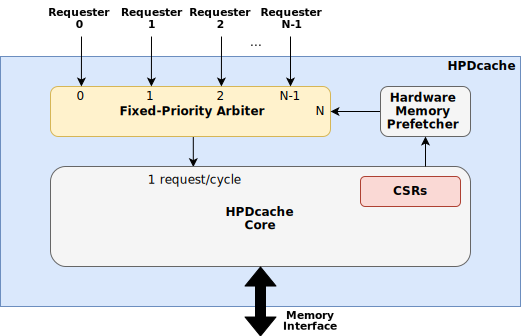
\includegraphics[width=\textwidth]{hpdcache_request_arbiter.pdf}
  \caption{\figlabel{dcache_req_arb}High-Level View of the HPDcache Sub-System}
\end{figure}

\newpage
\section{List of features}

\begin{itemize}[itemsep=0em]
\item Support for multiple outstanding requests per requester.
\item Support for multiple outstanding read misses and writes to memory.
\item Processes one request per cycle.
\item Any given requester can access 1 to 32 bytes of a cacheline per cycle.
\item Reduced energy consumption by limiting the number of RAMs consulted per request.
\item Fixed priority arbiter between requesters: the requester port with the lowest index has the highest priority.
\item Non-allocate, write-through policy.
\item Hardware write-buffer to mask the latency of write acknowledgements from the memory system.
\item Internal, configurable, hardware, memory-prefetcher that supports up to 4 simultaneous prefetching streams.
\item Compliance with \ac{RVWMO}.
  \begin{itemize}
  \item For address-overlapping transactions, the cache guarantees that these are committed in the order in which they are consumed from the requesters.
  \item For non-address-overlapping transactions, the cache may execute them in an out-of-order fashion to improve performance.
  \end{itemize}
\item Support for \acp{CMO}: cache invalidation operations, and memory fences for multi-core synchronisation. Cache invalidation operations support the ones defined in the RISC-V CMO Standard.
\item Memory-mapped \acp{CSR} for runtime configuration of the cache, status and performance monitoring.
\item Ready-Valid, 8 channels (4 request/4 response), interface to the memory. This interface, cache memory interface (CMI), can be easily adapted to mainstream \ac{NoC} interfaces like \acs{AMBA} AXI~\cite{arm_amba_2017}.
\item An adapter for interfacing with AXI5 is provided.
\end{itemize}

\newpage
\section{Synthesis-time (static) Configuration Parameters}

The \ac{HPDcache} has several static configuration parameters.
These parameters must be defined at compilation/synthesis.

\Tabref{dcache_parameters} summarizes the list of parameters that can be set when integrating the \ac{HPDcache}.
In \apxref{implementations}, we describe different systems where the \ac{HPDcache} was integrated, and we list the parameters used in those implementations.

\begin{table}[h!]
\begin{center}
\caption{HPDcache synthesis-time parameters}%
\tablabel{dcache_parameters}
{\footnotesize%
\begin{tabular}{p{.4\textwidth}p{.6\textwidth}}
\toprule%
$\mathsf{CONF\_DCACHE\_PA\_WIDTH}$ &%
Physical address width (in bits) \\
\midrule%
$\mathsf{CONF\_DCACHE\_WORD\_WIDTH}$ &%
Width (in bits) of a data word\\
\midrule%
$\mathsf{CONF\_DCACHE\_REQ\_WORDS}$ &%
Number of words in the data channels from/to requesters \\
\midrule%
$\mathsf{CONF\_DCACHE\_REQ\_TRANS\_ID\_WIDTH}$ &%
Width (in bits) of the transaction ID from requesters \\
\midrule%
$\mathsf{CONF\_DCACHE\_REQ\_SRC\_ID\_WIDTH}$ &%
Width (in bits) of the source ID from requesters \\
\midrule%
$\mathsf{CONF\_DCACHE\_SETS}$ &%
Number of sets \\
\midrule%
$\mathsf{CONF\_DCACHE\_WAYS}$ &%
Number of ways (associativity) \\
\midrule%
$\mathsf{CONF\_DCACHE\_CL\_WORDS}$ &%
Number of words in a cacheline\\
\midrule%
$\mathsf{CONF\_DCACHE\_WBUF\_DIR\_ENTRIES}$ &%
Number of entries in the directory of the write buffer \\
\midrule%
$\mathsf{CONF\_DCACHE\_WBUF\_DATA\_ENTRIES}$ &%
Number of entries in the data part of the write buffer \\
\midrule%
$\mathsf{CONF\_DCACHE\_WBUF\_WORDS}$ &%
Number of data words per entry in the write buffer \\
\midrule%
$\mathsf{CONF\_DCACHE\_WBUF\_TIMECNT\_WIDTH}$ &%
Width (in bits) of the time counter in write buffer entries \\
\midrule%
$\mathsf{CONF\_DCACHE\_RTAB\_ENTRIES}$ &%
Number of entries in the replay table \\
\midrule%
$\mathsf{CONF\_DCACHE\_MSHR\_SETS}$ &%
Number of sets in the \ac{MSHR} \\
\midrule%
$\mathsf{CONF\_DCACHE\_MSHR\_WAYS}$ &%
Number of ways (associativity) in the \ac{MSHR} \\
\midrule%
$\mathsf{CONF\_DCACHE\_MEM\_WORDS}$ &%
Number of words in the data channels from/to the memory interface \\
\midrule%
$\mathsf{CONF\_DCACHE\_MEM\_ID\_WIDTH}$ &%
Width (in bits) of the transaction ID from the memory interface \\
\end{tabular}}
\end{center}
\end{table}

Some parameters are not directly related with functionality (\tabref{dcache_physical_parameters}).
Instead, they allow adapting the \ac{HPDcache} to physical constraints in the target technology node.
Generally, these control the mapping to SRAM macros..
Depending on the technology, some dimensions are a more efficient than others (in terms of area, power, and performance).
These also need to be provided by the user at synthesis-time.

\begin{table}[h!]
\begin{center}
\caption{HPDcache synthesis-time physical parameters}%
\tablabel{dcache_physical_parameters}
{\footnotesize%
\begin{tabular}{p{.42\textwidth}p{.58\textwidth}}
\toprule%
$\mathsf{CONF\_DCACHE\_MSHR\_WAYS\_PER\_RAM\_WORD}$ &%
Number of ways in the same MSHR SRAM word\\
\midrule%
$\mathsf{CONF\_DCACHE\_MSHR\_SETS\_PER\_RAM}$ &%
Number of sets per RAM macro in the MSHR array of the cache\\
\midrule%
$\mathsf{CONF\_DCACHE\_DATA\_WAYS\_PER\_RAM\_WORD}$ &%
Number of ways in the same CACHE data SRAM word\\
\midrule%
$\mathsf{CONF\_DCACHE\_DATA\_SETS\_PER\_RAM}$ &%
Number of sets per RAM macro in the DATA array of the cache\\
\midrule%
$\mathsf{CONF\_DCACHE\_ACCESS\_WORDS}$ &%
Number of words of a given SET that can be accessed simultaneously from the CACHE data array \\
\tablabel{dcache_technology_dependent_parameters}
\end{tabular}}
\end{center}
\end{table}

Several internal configuration values are computed from the above ones.
\Tabref{dcache_internal_parameters} has a non-complete list of these internal configuration values that may be mentioned in the remainder of this document.

\begin{table}[h!]
\begin{center}
\caption{HPDcache internal parameters}%
\tablabel{dcache_internal_parameters}
{\footnotesize%
\begin{tabular}{p{.35\textwidth}p{.65\textwidth}}
\toprule%
\multirow{2}{*}{$\mathsf{DCACHE\_CL\_WIDTH}$}%
& Width (in bits) of a cacheline\\%
& $\mathsf{CONF\_DCACHE\_CL\_WORDS~\times~CONF\_DCACHE\_WORD\_WIDTH}$\\
\midrule%
\multirow{2}{*}{$\mathsf{DCACHE\_NLINE\_WIDTH}$}%
& Width (in bits) of the CACHELINE index part of the address\\%
& $\mathsf{CONF\_DCACHE\_PA\_WIDTH - log_2(DCACHE\_CL\_WIDTH/8)}$\\
\midrule%
\multirow{2}{*}{$\mathsf{DCACHE\_SET\_WIDTH}$}%
& Width (in bits) of the SET part of the address \\%
& $\mathsf{log_2(CONF\_DCACHE\_SETS)}$ \\
\midrule%
\multirow{2}{*}{$\mathsf{DCACHE\_TAG\_WIDTH}$}%
& Width (in bits) of the TAG part of the address\\%
& $\mathsf{DCACHE\_NLINE\_WIDTH - DCACHE\_SET\_WIDTH}$\\
\midrule%
\multirow{2}{*}{$\mathsf{DCACHE\_WBUF\_WIDTH}$}%
& Width (in bits) of an entry in the write-buffer\\%
& $\mathsf{CONF\_DCACHE\_WBUF\_WORDS~\times~CONF\_DCACHE\_WORD\_WIDTH}$\\
\end{tabular}}
\end{center}
\end{table}


\chapter{Interfaces and Communication Protocols}
\minitoc
\newpage

\section{Global Signals}
\seclabel{if_global_signals}

\begin{table}[h!]
\caption{Global signals}%
\tablabel{if_global_signals}
{\footnotesize%
\begin{tabular}{p{.21\linewidth}p{.15\linewidth}p{.64\linewidth}}
  \toprule
  \textbf{Signal}
  & \textbf{Source}
  & \textbf{Description} \\
  \midrule
  $\mathsf{CLK\_I}$
  & Clock source
  & Global clock signal.
  The \ac{HPDcache} is synchronous to the rising-edge of the clock.\\
  \midrule
  $\mathsf{RST\_NI}$
  & Reset source
  & Global reset signal.
  Asynchronous, active LOW, reset signal.\\
  \midrule
  $\mathsf{WBUF\_FLUSH\_I}$
  & System
  & Force the write-buffer to send all pending writes.
  Active HIGH, one-cycle, pulse signal.
  Synchronous to $\mathsf{CLK\_I}$.\\
  \midrule
  $\mathsf{WBUF\_EMPTY\_O}$
  & System
  & Indicates if the write-buffer is empty (there is no pending write transactions).
  When this signal is set to 1, the write-buffer is empty.\\
\end{tabular}}
\end{table}

\clearpage

\section{Requesters' Request/Response Interface}

This section describes the interfaces between the requesters and the \ac{HPDcache}.

All these interfaces are synchronous to the rising edge of the global clock $\mathsf{CLK\_I}$ (\secref{if_global_signals})


\subsection{Signal Descriptions}
\seclabel{if_requester_desc}

\begin{table}[h!]
\caption{Request channel signals}%
\tablabel{if_req}
{\footnotesize%
\begin{tabular}{p{.38\linewidth}p{.07\linewidth}p{.55\linewidth}}
  \toprule
  \textbf{Signal}
  & \textbf{Source}
  & \textbf{Description} \\
  \midrule
  $\mathsf{DCACHE\_REQ\_VALID}$
  & Requester
  & Indicates that the channel is signaling a valid request.
  See \secref{if_valid_ready}.\\
  \midrule
  $\mathsf{DCACHE\_REQ\_READY}$
  & Cache
  & Indicates that the cache is ready to accept a request.
  See \secref{if_valid_ready}.\\
  \midrule
  $\mathsf{DCACHE\_REQ\_ADDR}$
  & Requester
  & Target physical address of the request.
  The address shall be aligned to the $\mathsf{DCACHE\_REQ\_SIZE}$ field.
  See \secref{if_addr_data_alignment}.\\
  \midrule
  $\mathsf{DCACHE\_REQ\_OP}$
  & Requester
  & Indicates the type of operation to be performed.
  See \secref{if_req_op}.\\
  \midrule
  $\mathsf{DCACHE\_REQ\_WDATA}$
  & Requester
  & Write data (little-endian).
  It shall be naturally aligned to the address.
  See \secref{if_addr_data_alignment}.\\
  \midrule
  $\mathsf{DCACHE\_REQ\_BE}$
  & Requester
  & Byte-enable for write data (little-endian).
  It shall be naturally aligned to the address.
  See \secref{if_addr_data_alignment}.\\
  \midrule
  $\mathsf{DCACHE\_REQ\_SIZE}$
  & Requester
  & Indicate the size of the access.
  The size is encoded as the power-of-two of the number of bytes (e.g. 0 is $\mathsf{2^0~=~1}$, 5 is $\mathsf{2^5~=~32}$).\\
  \midrule
  $\mathsf{DCACHE\_REQ\_UNCACHEABLE}$
  & Requester
  & Indicates whether the access needs to be cached (unset) or not (set).
  Uncacheable accesses are directly forwarded to the memory.
  See \secref{if_req_uncacheable}.\\
  \midrule
  $\mathsf{DCACHE\_REQ\_SID}$
  & Requester
  & The identification tag for the requester.
  It shall be identical to the index of the request port binded to that requester.
  See \secref{if_req_sid}.\\
  \midrule
  $\mathsf{DCACHE\_REQ\_TID}$
  & Requester
  & The identification tag for the request.
  A requester can issue multiple requests.
  The corresponding response from the cache will return this TID.
  See \secref{if_req_tid}.\\
  \midrule
  $\mathsf{DCACHE\_REQ\_NEED\_RSP}$
  & Requester
  & The identification tag for the request.
  Indicates whether the request needs a response from the cache.
  When unset, the cache will not issue a response for the corresponding request.
  See \secref{if_req_need_rsp}.\\
\end{tabular}}
\end{table}

\begin{table}[h!]
\caption{Response channel signals}%
\tablabel{if_rsp}
{\footnotesize%
\begin{tabular}{p{.38\linewidth}p{.07\linewidth}p{.55\linewidth}}
  \toprule
  \textbf{Signal}
  & \textbf{Source}
  & \textbf{Description} \\
  \midrule
  $\mathsf{DCACHE\_RSP\_VALID}$
  & Cache
  & Indicates that the channel is signaling a valid response.
  See \secref{if_valid_ready}.\\
  \midrule
  $\mathsf{DCACHE\_RSP\_RDATA}$
  & Cache
  & Response read data.
  It shall be naturally aligned to the request address.
  See \secref{if_addr_data_alignment}.\\
  \midrule
  $\mathsf{DCACHE\_RSP\_SID}$
  & Cache
  & The identification tag for the requester.
  It corresponds to the SID transferred with the request.
  See \secref{if_req_sid}.\\
  \midrule
  $\mathsf{DCACHE\_RSP\_TID}$
  & Cache
  & The identification tag for the request.
  It corresponds to the TID transferred with the request.
  See \secref{if_req_tid}.\\
  \midrule
  $\mathsf{DCACHE\_RSP\_ERROR}$
  & Cache
  & Indicates whether there was an error condition while processing the request.
  See \secref{if_rsp_error}.\\
\end{tabular}}
\end{table}

\clearpage
\section{Memory Request/Response Interfaces}
\seclabel{if_mem_desc}

This section describes the interfaces between the \ac{HPDcache} and the \ac{NoC}/memory.

All these interfaces are synchronous to the rising edge of the global clock $\mathsf{CLK\_I}$ (\secref{if_global_signals})

\subsection{Signal Descriptions}

\begin{table}[h!]
\caption{Memory miss read request channel signals}%
\tablabel{if_mem_miss_req}
{\footnotesize%
\begin{tabular}{p{.38\linewidth}p{.07\linewidth}p{.55\linewidth}}
  \toprule
  \textbf{Signal}
  & \textbf{Source}
  & \textbf{Description} \\
  \midrule
  $\mathsf{MEM\_REQ\_MISS\_READ\_VALID}$
  & Cache
  & Indicates that the channel is signaling a valid request.\\
  \midrule
  $\mathsf{MEM\_REQ\_MISS\_READ\_READY}$
  & NoC
  & Indicates that the \ac{NoC} is ready to accept a request.\\
  \midrule
  $\mathsf{MEM\_REQ\_MISS\_READ\_ADDR}$
  & Cache
  & Target physical address of the request.
  The address shall be aligned to the $\mathsf{MEM\_REQ\_MISS\_READ\_SIZE}$ field.
  See \secref{if_addr_data_alignment}.\\
  \midrule
  $\mathsf{MEM\_REQ\_MISS\_READ\_LEN}$
  & Cache
  & Indicates the number of transfers in a burst minus one.
  \textbf{In this interface, for this version, this number is always 0 (one transfer)}.
  \textbf{However, bigger values may be used in the future. Thus, it should be decoded}.\\
  \midrule
  $\mathsf{MEM\_REQ\_MISS\_READ\_SIZE}$
  & Cache
  & Indicate the size of the access.
  The size is encoded as the power-of-two of the number of bytes.
  \textbf{In the current design implementation, the size value is equal to $\mathbf{log_2(DCACHE\_CL\_WIDTH/8)}$}.
  \textbf{However, smaller values may be used in the future. Thus, it should be decoded}.\\
  \midrule
  $\mathsf{MEM\_REQ\_MISS\_READ\_ID}$
  & Cache
  & The identification tag for the request\\
  \midrule
  $\mathsf{MEM\_REQ\_MISS\_READ\_COMMAND}$
  & Cache
  & Indicates the type of operation to be performed.
  \textbf{This interface only issues READ operations}.\\
  \midrule
  $\mathsf{MEM\_REQ\_MISS\_READ\_ATOMIC}$
  & Cache
  & In case of atomic operations, it indicates its type.
  \textbf{In this interface, this signal is not used, thus its value shall be ignored}.\\
  \midrule
  $\mathsf{MEM\_REQ\_MISS\_READ\_CACHEABLE}$
  & Cache
  & This is a hint for the cache hierarchy in the system.
  It indicates if the request can be allocated by the cache hierarchy.
  That is, data can be prefetched from memory or can be reused for multiple read transactions.
  \textbf{This bit is always set in this interface}.\\
\end{tabular}}
\end{table}

\begin{table}[h!]
\caption{Memory miss read response channel signals}%
\tablabel{if_mem_miss_rsp}
{\footnotesize%
\begin{tabular}{p{.38\linewidth}p{.07\linewidth}p{.55\linewidth}}
  \toprule
  \textbf{Signal}
  & \textbf{Source}
  & \textbf{Description} \\
  \midrule
  $\mathsf{MEM\_RESP\_MISS\_READ\_VALID}$
  & NoC
  & Indicates that the channel is signaling a valid response.\\
  \midrule
  $\mathsf{MEM\_RESP\_MISS\_READ\_READY}$
  & Cache
  & Indicates that the cache is ready to accept a response.\\
  \midrule
  $\mathsf{MEM\_RESP\_MISS\_READ\_ERROR}$
  & NoC
  & Indicates whether there was an error condition while processing the request.\\
  \midrule
  $\mathsf{MEM\_RESP\_MISS\_READ\_ID}$
  & NoC
  & The identification tag for the request.
  It corresponds to the ID transferred with the request.
  See \secref{if_addr_data_alignment}.\\
  \midrule
  $\mathsf{MEM\_RESP\_MISS\_READ\_DATA}$
  & NoC
  & Response read data.
  It shall be naturally aligned to the request address.
  See \secref{if_addr_data_alignment}.\\
  \midrule
  $\mathsf{MEM\_RESP\_MISS\_READ\_LAST}$
  & NoC
  & Indicates the last transfer in a read response burst.\\
\end{tabular}}
\end{table}

\clearpage
\begin{table}[h!]
\caption{Memory write-buffer write request channel signals}%
\tablabel{if_mem_wbuf_req}
{\footnotesize%
\begin{tabular}{p{.38\linewidth}p{.07\linewidth}p{.55\linewidth}}
  \toprule
  \textbf{Signal}
  & \textbf{Source}
  & \textbf{Description} \\
  \midrule
  $\mathsf{MEM\_REQ\_WBUF\_WRITE\_VALID}$
  & Cache
  & Indicates that the channel is signaling a valid request.\\
  \midrule
  $\mathsf{MEM\_REQ\_WBUF\_WRITE\_READY}$
  & NoC
  & Indicates that the cache is ready to accept a response.\\
  \midrule
  $\mathsf{MEM\_REQ\_WBUF\_WRITE\_ADDR}$
  & Cache
  & Target physical address of the request.
  The address shall be aligned to the $\mathsf{MEM\_REQ\_WBUF\_WRITE\_SIZE}$ field.
  See \secref{if_addr_data_alignment}.\\
  \midrule
  $\mathsf{MEM\_REQ\_WBUF\_WRITE\_LEN}$
  & Cache
  & Indicates the number of transfers in a burst minus one.
  \textbf{In this interface, this number is always 0 (one transfer)}.
  \textbf{However, bigger values may be used in the future.
  Thus, it should be decoded}.\\
  \midrule
  $\mathsf{MEM\_REQ\_WBUF\_WRITE\_SIZE}$
  & Cache
  & Indicate the size of the access.
  The size is encoded as the power-of-two of the number of bytes.
  \textbf{In this interface, the size shall be less or equal to $\mathbf{log_2(CONF\_DCACHE\_WBUF\_WORDS)}$}.\\
  \midrule
  $\mathsf{MEM\_REQ\_WBUF\_WRITE\_ID}$
  & Cache
  & The identification tag for the request.\\
  \midrule
  $\mathsf{MEM\_REQ\_WBUF\_WRITE\_COMMAND}$
  & Cache
  & Indicates the type of operation to be performed.
  \textbf{In this interface, this signal is always a WRITE operation}.\\
  \midrule
  $\mathsf{MEM\_REQ\_WBUF\_WRITE\_ATOMIC}$
  & Cache
  & In case of atomic operations, it indicates its type.
  \textbf{In this interface, this signal is not used, thus its value shall be ignored}.\\
  \midrule
  $\mathsf{MEM\_REQ\_WBUF\_WRITE\_CACHEABLE}$
  & Cache
  & This is a hint for the cache hierarchy in the system.
  It indicates if the write is bufferable by the cache hierarchy.
  This means that the write must be visible in a timely manner at the final destination.
  However, write responses can be obtained from an intermediate point.
  \textbf{This bit is always set in this interface}.\\
\end{tabular}}
\end{table}

\begin{table}[h!]
\caption{Memory write-buffer write data request channel signals}%
\tablabel{if_mem_wbuf_data}
{\footnotesize%
\begin{tabular}{p{.38\linewidth}p{.07\linewidth}p{.55\linewidth}}
  \toprule
  \textbf{Signal}
  & \textbf{Source}
  & \textbf{Description} \\
  \midrule
  $\mathsf{MEM\_REQ\_WBUF\_WRITE\_DATA\_VALID}$
  & Cache
  & Indicates that the channel is transferring a valid data.\\
  \midrule
  $\mathsf{MEM\_REQ\_WBUF\_WRITE\_DATA\_READY}$
  & NoC
  & Indicates that the target is ready to accept the data.\\
  \midrule
  $\mathsf{MEM\_REQ\_WBUF\_WRITE\_DATA\_WDATA}$
  & Cache
  & Request write data.
  It shall be naturally aligned to the request address.
  See \secref{if_addr_data_alignment}.\\
  \midrule
  $\mathsf{MEM\_REQ\_WBUF\_WRITE\_DATA\_BE}$
  & Cache
  & Request write byte-enable.
  It shall be naturally aligned to the request address.
  See \secref{if_addr_data_alignment}.\\
  \midrule
  $\mathsf{MEM\_REQ\_WBUF\_WRITE\_DATA\_LAST}$
  & Cache
  & Indicates the last transfer in a write request burst.\\
\end{tabular}}
\end{table}

\begin{table}[h!]
\caption{Memory write-buffer write response channel signals}%
\tablabel{if_mem_wbuf_rsp}
{\footnotesize%
\begin{tabular}{p{.38\linewidth}p{.07\linewidth}p{.55\linewidth}}
  \toprule
  \textbf{Signal}
  & \textbf{Source}
  & \textbf{Description} \\
  \midrule
  $\mathsf{MEM\_RESP\_WBUF\_WRITE\_VALID}$
  & NoC
  & Indicates that the channel is transferring a valid write acknowledgement.\\
  \midrule
  $\mathsf{MEM\_RESP\_WBUF\_WRITE\_READY}$
  & Cache
  & Indicates that the cache is ready to accept the acknowledgement.\\
  \midrule
  $\mathsf{MEM\_RESP\_WBUF\_WRITE\_IS\_ATOMIC}$
  & NoC
  & Indicates whether the atomic operation was successfully processed (atomically).
  \textbf{The value in this signal is ignored in this interface}.\\
  \midrule
  $\mathsf{MEM\_RESP\_WBUF\_WRITE\_ERROR}$
  & NoC
  & Indicates whether there was an error condition while processing the request.\\
  \midrule
  $\mathsf{MEM\_RESP\_WBUF\_WRITE\_ID}$
  & NoC
  & The identification tag for the request.
  It corresponds to the ID transferred with the request.\\
\end{tabular}}
\end{table}

\clearpage

\begin{table}[h!]
\caption{Memory read uncached request channel signals}
\tablabel{if_mem_uc_read}
{\footnotesize%
\begin{tabular}{p{.38\linewidth}p{.07\linewidth}p{.55\linewidth}}
  \toprule
  \textbf{Signal}
  & \textbf{Source}
  & \textbf{Description} \\
  \midrule
  $\mathsf{MEM\_REQ\_UC\_READ\_VALID}$
  & Cache
  & Indicates that the channel is signaling a valid request.\\
  \midrule
  $\mathsf{MEM\_REQ\_UC\_READ\_READY}$
  & NoC
  & Indicates that the \ac{NoC} is ready to accept a request.\\
  \midrule
  $\mathsf{MEM\_REQ\_UC\_READ\_ADDR}$
  & Cache
  & Target physical address of the request.
  The address shall be aligned to the $\mathsf{MEM\_REQ\_MISS\_READ\_SIZE}$ field.
  See \secref{if_addr_data_alignment}.\\
  \midrule
  $\mathsf{MEM\_REQ\_UC\_READ\_LEN}$
  & Cache
  & Indicates the number of transfers in a burst minus one.
  \textbf{In this interface, this number is always 0 (one transfer)}.\\
  \midrule
  $\mathsf{MEM\_REQ\_UC\_READ\_SIZE}$
  & Cache
  & Indicate the size of the access.
  The size is encoded as the power-of-two of the number of bytes.\\
  \midrule
  $\mathsf{MEM\_REQ\_UC\_READ\_ID}$
  & Cache
  & The identification tag for the request\\
  \midrule
  $\mathsf{MEM\_REQ\_UC\_READ\_COMMAND}$
  & Cache
  & Indicates the type of operation to be performed.
  \textbf{In this interface, this signal is always a READ operation}.\\
  \midrule
  $\mathsf{MEM\_REQ\_UC\_READ\_ATOMIC}$
  & Cache
  & In case of atomic operations, it indicates its type.
  \textbf{In this interface, this signal is not used, thus its value shall be ignored}.\\
  \midrule
  $\mathsf{MEM\_REQ\_UC\_READ\_CACHEABLE}$
  & Cache
  & This is a hint for the cache hierarchy in the system.
  It indicates if the request can be allocated by the cache hierarchy.
  That is, data can be prefetched from memory or can be reused for multiple read transactions.
  \textbf{This bit is always unset in this interface.
  Thus data shall come from the final destination}.\\
\end{tabular}}
\end{table}

\begin{table}[h!]
\caption{Memory read uncached response channel signals}%
\tablabel{if_mem_uc_read_rsp}
{\footnotesize%
\begin{tabular}{p{.38\linewidth}p{.07\linewidth}p{.55\linewidth}}
  \toprule
  \textbf{Signal}
  & \textbf{Source}
  & \textbf{Description} \\
  & & Signals are identical that for the miss response channel signals.
\end{tabular}}
\end{table}

\clearpage

\begin{table}[h!]
\caption{Memory write uncached request channel signals}%
\tablabel{if_mem_uc_write}
{\footnotesize%
\begin{tabular}{p{.38\linewidth}p{.07\linewidth}p{.55\linewidth}}
  \toprule
  \textbf{Signal}
  & \textbf{Source}
  & \textbf{Description} \\
  \midrule
  $\mathsf{MEM\_REQ\_UC\_WRITE\_VALID}$
  & Cache
  & Indicates that the channel is signaling a valid request.\\
  \midrule
  $\mathsf{MEM\_REQ\_UC\_WRITE\_READY}$
  & NoC
  & Indicates that the cache is ready to accept a response.\\
  \midrule
  $\mathsf{MEM\_REQ\_UC\_WRITE\_ADDR}$
  & Cache
  & Target physical address of the request.
  The address shall be aligned to the $\mathsf{MEM\_REQ\_UC\_WRITE\_SIZE}$ field.
  See \secref{if_addr_data_alignment}\\
  \midrule
  $\mathsf{MEM\_REQ\_UC\_WRITE\_LEN}$
  & Cache
  & Indicates the number of transfers in a burst minus one.
  \textbf{In the current \acs{HPDcache} implementation, this number is always 0 (one transfer)}.\\
  \midrule
  $\mathsf{MEM\_REQ\_UC\_WRITE\_SIZE}$
  & Cache
  & Indicate the size of the access.
  The size is encoded as the power-of-two of the number of bytes.\\
  \midrule
  $\mathsf{MEM\_REQ\_UC\_WRITE\_ID}$
  & Cache
  & The identification tag for the request.\\
  \midrule
  $\mathsf{MEM\_REQ\_UC\_WRITE\_COMMAND}$
  & Cache
  & Indicates the type of operation to be performed.
  \textbf{In this interface, this signal is either a WRITE or an ATOMIC operation}.\\
  \midrule
  $\mathsf{MEM\_REQ\_UC\_WRITE\_ATOMIC}$
  & Cache
  & In case of atomic operations, it indicates its type.\\
  \midrule
  $\mathsf{MEM\_REQ\_UC\_WRITE\_CACHEABLE}$
  & Cache
  & This is a hint for the cache hierarchy in the system.
  It indicates if the write is bufferable by the cache hierarchy.
  This means that the write must be visible in a timely manner at the final destination.
  However, write responses can be obtained from an intermediate point.
  \textbf{This bit is always unset in this interface (thus transactions are non-bufferable, and the response shall come from the final destination)}.\\
\end{tabular}}
\end{table}

\begin{table}[h!]
\caption{Memory write data uncached request channel signals}%
\tablabel{if_mem_uc_write_data}
{\footnotesize%
\begin{tabular}{p{.38\linewidth}p{.07\linewidth}p{.55\linewidth}}
  \toprule
  \textbf{Signal}
  & \textbf{Source}
  & \textbf{Description} \\
  & & Signals are identical to those for the write data request channel signals.
\end{tabular}}
\end{table}

\begin{table}[h!]
\caption{Memory write uncached response channel signals}%
\tablabel{if_mem_uc_write_rsp}
{\footnotesize%
\begin{tabular}{p{.38\linewidth}p{.07\linewidth}p{.55\linewidth}}
  \toprule
  \textbf{Signal}
  & \textbf{Source}
  & \textbf{Description} \\
  \midrule
  $\mathsf{MEM\_RESP\_UC\_WRITE\_VALID}$
  & NoC
  & Indicates that the channel is transferring a valid write acknowledgement.\\
  \midrule
  $\mathsf{MEM\_RESP\_UC\_WRITE\_READY}$
  & Cache
  & Indicates that the cache is ready to accept the acknowledgement.\\
  \midrule
  $\mathsf{MEM\_RESP\_UC\_WRITE\_IS\_ATOMIC}$
  & NoC
  & Indicates whether the atomic operation was successfully processed (atomically).\\
  \midrule
  $\mathsf{MEM\_RESP\_UC\_WRITE\_ERROR}$
  & NoC
  & Indicates whether there was an error condition while processing the request.\\
  \midrule
  $\mathsf{MEM\_RESP\_UC\_WRITE\_ID}$
  & NoC
  & The identification tag for the request.
  It corresponds to the ID transferred with the request.\\
\end{tabular}}
\end{table}

\section{Interfaces' requirements}

This section describes the basic protocol transaction requirements for the different interfaces in the \ac{HPDcache}.

\subsection{Valid/ready handshake process}%
\seclabel{if_valid_ready}

All interfaces in the \ac{HPDcache} use a \textbf{VALID}/\textbf{READY} handshake process to transfer a payload between a source and a destination.
The payload contains the address, data and control information.

As a reminder, the interfaces in the \ac{HPDcache} are the following:
\begin{itemize}
  \item Requesters' request interface (\tabref{if_req});
  \item Requesters' response interface (\tabref{if_rsp});
  \item Memory miss read request interface (\tabref{if_mem_miss_req});
  \item Memory miss read response interface (\tabref{if_mem_miss_rsp});
  \item Memory write-buffer write request interface (\tabref{if_mem_wbuf_req});
  \item Memory write-buffer write data request interface (\tabref{if_mem_wbuf_data});
  \item Memory write-buffer write response interface (\tabref{if_mem_wbuf_rsp});
  \item Memory uncached read request interface (\tabref{if_mem_uc_read});
  \item Memory uncached read response interface (\tabref{if_mem_uc_read_rsp});
  \item Memory uncached write request interface (\tabref{if_mem_uc_write});
  \item Memory uncached write data request interface (\tabref{if_mem_uc_write_data});
  \item Memory uncached write response interface (\tabref{if_mem_uc_write_rsp});
\end{itemize}

The source sets to 1 the \textbf{VALID} signal to indicate when the payload is available.
The destination sets to 1 the \textbf{READY} signal to indicate that it can accept that payload.
Transfer occurs only when both the \textbf{VALID} and \textbf{READY} signals are set to 1 on the next rising edge of the clock.

A source is not permitted to wait until \textbf{READY} is set to 1 before setting \textbf{VALID} to 1.

A destination may or not wait for \textbf{VALID} to set the \textbf{READY} to 1 (\figref{valid_ready_scenarios} (a) \& (c)). In other words, a destination may set \textbf{READY} to 1 before an actual transfer is available (\figref{valid_ready_scenarios} (a)).

When \textbf{VALID} is set to 1, the source must keep it that way until the handshake occurs.
This is, at the next rising edge when both \textbf{VALID} and \textbf{READY} (from the destination) are set to 1. In other words, a source cannot retire a pending \textbf{VALID} transfer (\figref{valid_ready_scenarios} (b)).

After an effective transfer (\textbf{VALID} and \textbf{READY} set to 1), the source may keep \textbf{VALID} set to 1 in the next cycle to signal a new transfer (with a new payload).
In the same manner, the destination may keep \textbf{READY} set to 1 if it can accept a new transfer.
This allows back-to-back transfers, with no idle cycles, between a source and a destination (\figref{valid_ready_scenarios} (d)).

All interfaces are synchronous to the rising edge of the same global clock (\tabref{if_global_signals}).

\begin{figure}[htbp]
  {\centering
  \begin{tabular}{cc}
    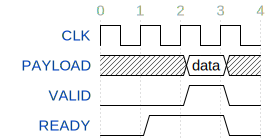
\includegraphics[height=10em]{wave_ready_before_valid.pdf}
    & 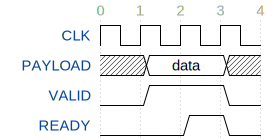
\includegraphics[height=10em]{wave_valid_before_ready.pdf} \\
    \textbf{(a)}
    & \textbf{(b)} \\
    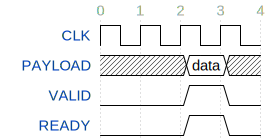
\includegraphics[height=10em]{wave_ready_when_valid.pdf}
    & 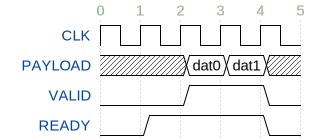
\includegraphics[height=10em]{wave_back_to_back.pdf} \\
    \textbf{(c)}
    & \textbf{(d)} \\
  \end{tabular}
  \caption{\figlabel{valid_ready_scenarios}VALID/READY scenarios}}
\end{figure}

\paragraph{Requesters' reponse interface}\mbox{}

In the case of the requesters' response interfaces, there is a particularity.
For these interfaces, it is assumed that the \textbf{READY} signal is always set to 1.
That is why the \textbf{READY} signal is not actually implemented on those interfaces.
In other words, the requester must unconditionally accept the response, when it arrives.


\subsection{Address, data and byte enable alignment}
\seclabel{if_addr_data_alignment}

\paragraph{Address alignment}\mbox{}

In all request interfaces (Requesters' request interface, Memory miss read request interface, Memory write-buffer write request interface, Memory uncached read request interface, Memory uncached write request interface), the address transfered (\textbf{ADDR}) shall be byte-aligned to the value of the corresponding \textbf{SIZE} signal in that interface.

Some examples are illustrated in \figref{req_addr_alignment}.
In the first case, the \textbf{SIZE} value is 2 (which corresponds to $2^2=4$ bytes).
Thus, the address must be a multiple of 4;
In the second case, \textbf{SIZE} value is 3.
Thus, the address must be a multiple of 8.
Finally, in the third case, \textbf{SIZE} value is 0.
Thus, there is no constraint on the address alignment.

\paragraph{Data alignment}\mbox{}

The data must be naturally aligned to the address (\textbf{ADDR}) and the maximum valid bytes of the transfer must be equal to $\mathsf{2^\mathbf{SIZE}}$.
This means that the first valid byte in the \textbf{DATA} signal must be at the indicated offset of the address.
Here, the offset corresponds to the least significant bits of the address, that allow to indicate a byte within the \textbf{DATA} word.
For example, if the \textbf{DATA} signal is 128 bits wide (16 bytes), then the offset corresponds to the first 4 bits of the \textbf{ADDR} signal.

Some examples are illustrated in \figref{req_addr_alignment}.
As illustrated, within the data word, only bytes in the range from the indicated offset in the address, to that offset plus $\mathsf{2^\mathbf{SIZE}}$ can contain valid data.
Other bytes must be ignored by the destination.

Additionally, within the range described above, the \textbf{BE} signal indicates which bytes within that range are actually valid.
Bytes in the \textbf{WDATA} signal where the \textbf{BE} signals are set to 0, must be ignored by the destination.

\paragraph{Byte Enable (BE) alignment}\mbox{}

The \textbf{BE} signal must be naturally aligned to the address (\textbf{ADDR}) and the number of bits set in this signal must be less or equal to $\mathsf{2^\mathbf{SIZE}}$.
This means that the first valid bit in the \textbf{BE} signal must be at the indicated offset of the address.
The offset is the same as the one explained above in the "Data alignment" paragraph.

Some examples are illustrated in \figref{req_addr_alignment}.
As illustrated, within the \textbf{BE} word, only bits in the range from the indicated offset in the address, to that offset plus $\mathsf{2^\mathbf{SIZE}}$ can be set.
Other bits outside that range must be set to 0.

\begin{figure}[tbp]
    \centering
    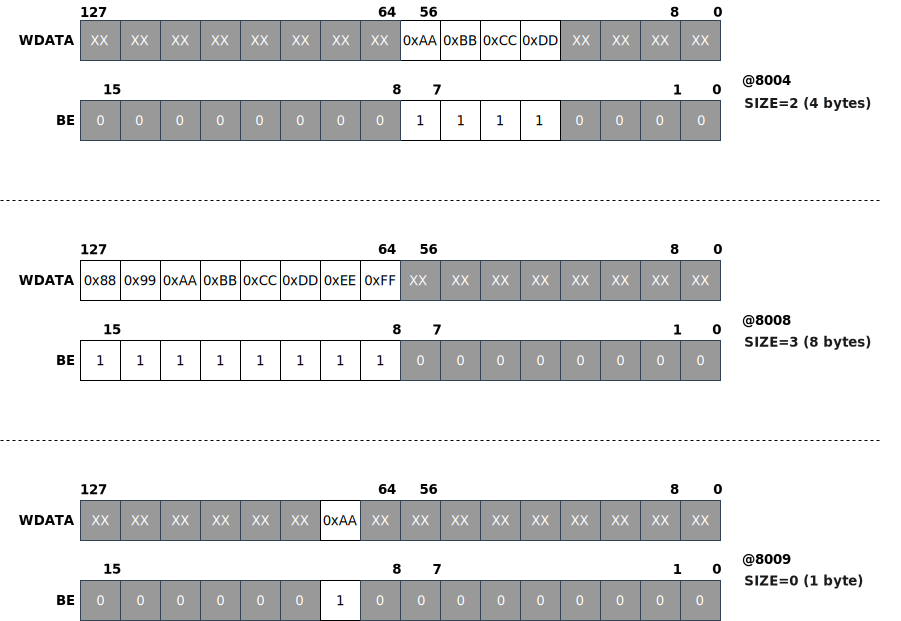
\includegraphics[width=\textwidth]{hpdcache_request_address_data_alignment.pdf}
    \caption{\figlabel{req_addr_alignment}Address, Data and Byte Enable Alignment in Requests}
\end{figure}


\clearpage
\section{Requesters interface attributes}%
\seclabel{if_req_attr}

\subsection{Type of operation}%
\seclabel{if_req_op}

A requester indicates the required operation on the 4-bit, $\mathsf{DCACHE\_REQ\_OP}$ signal.
The supported operation are detailed in \tabref{dcache_req_op}.

\begin{table}[h!]
\begin{center}
\caption{Request operation types}%
\tablabel{dcache_req_op}
{\footnotesize
\begin{tabular}{lll}
  \toprule
  \textbf{Mnemonic}
  & \textbf{Encoding}
  & \textbf{Type} \\
  \midrule
  $\mathsf{DCACHE\_REQ\_LOAD}$
  & 0b0000
  & Read operation \\
  \midrule
  $\mathsf{DCACHE\_REQ\_STORE}$
  & 0b0001
  & Write operation \\
  \midrule
  $\mathsf{DCACHE\_REQ\_AMO\_LR}$
  & 0b0100
  & Atomic Load-reserved operation \\
  \midrule
  $\mathsf{DCACHE\_REQ\_AMO\_SC}$
  & 0b0101
  & Atomic Store-conditional operation \\
  \midrule
  $\mathsf{DCACHE\_REQ\_AMO\_SWAP}$
  & 0b0110
  & Atomic SWAP operation \\
  \midrule
  $\mathsf{DCACHE\_REQ\_AMO\_ADD}$
  & 0b0111
  & Atomic integer ADD operation \\
  \midrule
  $\mathsf{DCACHE\_REQ\_AMO\_AND}$
  & 0b1000
  & Atomic bitwise AND operation \\
  \midrule
  $\mathsf{DCACHE\_REQ\_AMO\_OR}$
  & 0b1001
  & Atomic bitwise OR operation \\
  \midrule
  $\mathsf{DCACHE\_REQ\_AMO\_XOR}$
  & 0b1010
  & Atomic bitwise XOR operation \\
  \midrule
  $\mathsf{DCACHE\_REQ\_AMO\_MAX}$
  & 0b1011
  & Atomic integer signed MAX operation \\
  \midrule
  $\mathsf{DCACHE\_REQ\_AMO\_MAXU}$
  & 0b1100
  & Atomic integer unsigned MAX operation \\
  \midrule
  $\mathsf{DCACHE\_REQ\_AMO\_MIN}$
  & 0b1101
  & Atomic integer signed MIN operation \\
  \midrule
  $\mathsf{DCACHE\_REQ\_AMO\_MINU}$
  & 0b1110
  & Atomic integer unsigned MIN operation \\
  \midrule
  $\mathsf{DCACHE\_REQ\_CMO}$
  & 0b1111
  & \acf*{CMO} \\
\end{tabular}}
\end{center}
\end{table}

Load and store operations are normal read and write operations from/to the specified address.

Atomic operations are the ones specified in the Atomic (A) extension of the \citetitle{RISCV_spec}\cite{RISCV_spec}.
More details on how this cache implements them are found in \charef{amo}.

\acfp{CMO} are explained in \charef{cmo}


\subsection{Source identifier}
\seclabel{if_req_sid}

Each request identifies its source through the $\mathsf{DCACHE\_REQ\_SID}$ signal.
The $\mathsf{DCACHE\_REQ\_SID}$ signal shall be decoded when the $\mathsf{DCACHE\_REQ\_VALID}$ signal is set to 1.

The width of this signal is $\mathsf{CONF\_DCACHE\_REQ\_SRC\_ID\_WIDTH}$ (\tabref{dcache_parameters}) bits.

The \ac{HPDcache} reflects the value of the \textbf{SID} of the request into the corresponding \textbf{SID} of the response.

Each port must have an unique ID that corresponds to its number.
Each port is numbered from $\mathsf{0}$ to $\mathsf{N-1}$.
Port number $\mathsf{N}$ is dedicated to the hardware memory prefetcher.
This number shall be constant for a given port (requester).

The \ac{HPDcache} uses this information to route responses to the correct requester.


\subsection{Transaction identifier}
\seclabel{if_req_tid}

Each request identifies transactions through the $\mathsf{DCACHE\_REQ\_TID}$ signal.
The $\mathsf{DCACHE\_REQ\_TID}$ signal shall be decoded when the $\mathsf{DCACHE\_REQ\_VALID}$ signal is set to 1.

The width of this signal is $\mathsf{CONF\_DCACHE\_REQ\_TRANS\_ID\_WIDTH}$ bits (\tabref{dcache_parameters}).

This signal can contain any value from $\mathsf{0}$ to $\mathsf{2^{CONF\_DCACHE\_REQ\_TRANS\_ID\_WIDTH} - 1}$.

The \ac{HPDcache} forwards the value of the \textbf{TID} of the request into the \textbf{TID} of the corresponding response.

A requester can issue multiple transactions without waiting for earlier transactions to complete.
Because the \ac{HPDcache} can respond to these transactions in a different order than that of requests, the requester can use the \textbf{TID} to match the responses with respect to requests.

The ID of transactions is not necessarily unique.
A requester may reuse a given transaction ID for different transactions.
That is, even when some of these transactions are not yet completed.
In this case, when the requester starts multiple transactions with the same \textbf{TID}, the requester cannot match responses and requests.
As explained above, this is because the cache can respond out-of-order with respect to requests.


\subsection{Cacheability}
\seclabel{if_req_uncacheable}

This cache considers that the memory space is segmented.
A segment corresponds to an address range: a base address and an end address.
Some segments are cacheable and others not.
The \ac{HPDcache} needs to know which segments are cacheable to determine if for a given read request, it needs to replicate read data into the cache.

The request interface implements an uncacheable bit ($\mathsf{DCACHE\_REQ\_UNCACHEABLE}$).
When this bit is set, the access is considered uncacheable.
The $\mathsf{DCACHE\_REQ\_UNCACHEABLE}$ signal shall be decoded when the $\mathsf{DCACHE\_REQ\_VALID}$ signal is set to 1.

\begin{tcolorbox}[colback=red!10!white,
                  colframe=white!10!red,
                  title=\textbf{Important},
                  center, valign=top, halign=left,
                  center title,
                  width=.950\linewidth]
For a given address, the uncacheable attribute must be consistent between accesses.
The granularity is the cacheline.
In the event that the same address is accessed with different values in the uncacheable attribute, the behavior of the cache for that address is unpredictable.
\end{tcolorbox}


\subsection{Need response}%
\seclabel{if_req_need_rsp}

For any given request, a requester can set to 0 the bit $\mathsf{DCACHE\_REQ\_NEED\_RSP}$ to indicate that it does not wish a response for that request.
The $\mathsf{DCACHE\_REQ\_NEED\_RSP}$ signal shall be decoded when the $\mathsf{DCACHE\_REQ\_VALID}$ signal is set to 1.

When $\mathsf{DCACHE\_REQ\_NEED\_RSP}$ is set to 0, the \ac{HPDcache} processes the request but it does not send an acknowledge to the corresponding requester when the transaction is completed.


\subsection{Error response}%
\seclabel{if_rsp_error}

The response interface contains a single-bit $\mathsf{DCACHE\_RSP\_ERROR}$ signal.
This signal is set to 1 by the \ac{HPDcache} when some error condition occurred during the processing of the corresponding request.
The $\mathsf{DCACHE\_RSP\_ERROR}$ signal shall be decoded when the $\mathsf{DCACHE\_RSP\_VALID}$ signal is set to 1.

When the $\mathsf{DCACHE\_RSP\_ERROR}$ signal is set to 1 in the response, the effect of the corresponding request is undetermined.
In the case of \textbf{LOAD} or \textbf{AMOs} operations (see \secref{if_req_op}), the \textbf{RDATA} signal in the response does not contain any valid data.


\clearpage
\section{Memory interface attributes}

\subsection{Type of operation}%
\seclabel{if_mem_req_op}

\begin{table}[h!]
\begin{center}
\caption{Memory request operation types}%
\tablabel{dcache_mem_req_op}
{\footnotesize
\begin{tabular}{lll}
  \toprule
  \textbf{Mnemonic}
  & \textbf{Encoding}
  & \textbf{Type} \\
  \midrule
  $\mathsf{DCACHE\_MEM\_LOAD}$
  & 0b00
  & Read operation \\
  \midrule
  $\mathsf{DCACHE\_MEM\_STORE}$
  & 0b01
  & Write operation \\
  \midrule
  $\mathsf{DCACHE\_MEM\_ATOMIC}$
  & 0b10
  & Atomic operation \\
\end{tabular}}
\end{center}
\end{table}

Load and store operations are normal read and write operations from/to the specified address.

In case of an atomic operation request ($\mathsf{DCACHE\_MEM\_ATOMIC}$), the specific operation is specified in the $\mathsf{MEM\_REQ\_ATOMIC}$ signal.


\subsubsection{Atomic operations on the memory interface}

The supported atomic operations are listed in \tabref{dcache_mem_req_atop}.
These are transmitted in the $\mathsf{MEM\_REQ\_ATOMIC}$ signal.
Note that these operations are compatible with those in AXI.

\begin{table}[h!]
\begin{center}
\caption{Memory request atomic operation types}%
\tablabel{dcache_mem_req_atop}
{\footnotesize
\begin{tabular}{lll}
  \toprule
  \textbf{Mnemonic}
  & \textbf{Encoding}
  & \textbf{Type} \\
  \midrule
  $\mathsf{DCACHE\_MEM\_ATOMIC\_ADD}$
  & 0b0000
  & Atomic fetch-and-add operation \\
  \midrule
  $\mathsf{DCACHE\_MEM\_ATOMIC\_CLR}$
  & 0b0001
  & Atomic fetch-and-clear operation \\
  \midrule
  $\mathsf{DCACHE\_MEM\_ATOMIC\_SET}$
  & 0b0010
  & Atomic fetch-and-set operation \\
  \midrule
  $\mathsf{DCACHE\_MEM\_ATOMIC\_EOR}$
  & 0b0011
  & Atomic fetch-and-exclusive-or operation \\
  \midrule
  $\mathsf{DCACHE\_MEM\_ATOMIC\_SMAX}$
  & 0b0100
  & Atomic fetch-and-maximum (signed) operation \\
  \midrule
  $\mathsf{DCACHE\_MEM\_ATOMIC\_SMIN}$
  & 0b0101
  & Atomic fetch-and-minimum (signed) operation \\
  \midrule
  $\mathsf{DCACHE\_MEM\_ATOMIC\_UMAX}$
  & 0b0110
  & Atomic fetch-and-maximum (unsigned) operation \\
  \midrule
  $\mathsf{DCACHE\_MEM\_ATOMIC\_UMIN}$
  & 0b0111
  & Atomic fetch-and-minimum (unsigned) operation \\
  \midrule
  $\mathsf{DCACHE\_MEM\_ATOMIC\_SWAP}$
  & 0b1000
  & Atomic swap operation \\
  \midrule
  $\mathsf{DCACHE\_MEM\_ATOMIC\_LDEX}$
  & 0b1100
  & Load-exclusive operation \\
  \midrule
  $\mathsf{DCACHE\_MEM\_ATOMIC\_STEX}$
  & 0b1101
  & Store-exclusive operation \\
\end{tabular}}
\end{center}
\end{table}

\subsubsection{Operations used per interface}

As a reminder, the \ac{HPDcache} implements multiple (four) request interfaces to the memory:

\begin{itemize}
  \item Memory miss read request interface (\tabref{if_mem_miss_req});
  \item Memory write-buffer (wbuf) write request interface (\tabref{if_mem_wbuf_req});
  \item Memory uncached read request interface (\tabref{if_mem_uc_read});
  \item Memory uncached write request interface (\tabref{if_mem_uc_write});
\end{itemize}

\Tabref{dcache_mem_req_supported_op} indicates the type of operations that each of these four request interfaces can issue.

\begin{table}[!htbp]
\begin{center}
\caption{Supported operation types by request interfaces to the memory}%
\tablabel{dcache_mem_req_supported_op}
{\footnotesize
\begin{tabular}{ll}
  \toprule
  \textbf{Type}
  & \textbf{Interfaces}\\
  \midrule
  $\mathsf{MEM\_REQ\_LOAD}$
  &
  \begin{tabular}{l}
  - Memory miss read request;\\
  - Memory uncached read request.
  \end{tabular}
  \\
  \midrule
  $\mathsf{MEM\_REQ\_STORE}$
  &
  \begin{tabular}{l}
  - Memory write-buffer write request;\\
  - Memory uncached write request.
  \end{tabular}\\
  \midrule
  $\mathsf{MEM\_REQ\_ATOMIC}$
  &
  \begin{tabular}{l}
  - Memory uncached write request.
  \end{tabular}\\
\end{tabular}}
\end{center}
\end{table}


\subsubsection{Responses for read-modify-write atomic operations on the memory interface}

\begin{minipage}{\textwidth}
The requests listed below behave as a read-modify-write operations:
{\small\begin{itemize}[itemsep=0pt]
  \item $\mathsf{DCACHE\_MEM\_ATOMIC\_ADD}$
  \item $\mathsf{DCACHE\_MEM\_ATOMIC\_CLR}$
  \item $\mathsf{DCACHE\_MEM\_ATOMIC\_SET}$
  \item $\mathsf{DCACHE\_MEM\_ATOMIC\_EOR}$
  \item $\mathsf{DCACHE\_MEM\_ATOMIC\_SMAX}$
  \item $\mathsf{DCACHE\_MEM\_ATOMIC\_SMIN}$
  \item $\mathsf{DCACHE\_MEM\_ATOMIC\_UMAX}$
  \item $\mathsf{DCACHE\_MEM\_ATOMIC\_UMIN}$
  \item $\mathsf{DCACHE\_MEM\_ATOMIC\_SWAP}$
\end{itemize}}
\end{minipage}

These requests are forwarded to the memory through the uncached write request interface (\tabref{if_mem_uc_write}).
A particularity of these requests is that they generate two responses from the memory:
\begin{itemize}
  \item Old data value from memory is returned through the memory uncached read response interface (\tabref{if_mem_uc_read_rsp}).
  \item Write acknowledgement is returned through the memory uncached write response interface (\tabref{if_mem_uc_write_rsp}).
\end{itemize}

Both responses may arrive in any given order to the initiating \ac{HPDcache}.

Regarding errors, if any response has its ERROR signal set to 1 ($\mathsf{MEM\_RESP\_UC\_*\_ERROR}$), the \ac{HPDcache} considers that the operation was not completed.
It waits for both responses and it forwards an error response ($\mathsf{DCACHE\_RSP\_ERROR}$ is set to 1) to the corresponding requester on the \ac{HPDcache} requesters' side.


\subsubsection{Responses for exclusive load and store operations on the memory interface}

Exclusive load and store operations are issued as normal load and store operations on the memory uncached read request interface (\tabref{if_mem_uc_read}) and memory uncached write request interface (\tabref{if_mem_uc_write}), respectively.

Specific operation types are however used on these exclusive requests:
$\mathsf{DCACHE\_MEM\_ATOMIC\_LDEX}$ for loads; and $\mathsf{DCACHE\_MEM\_ATOMIC\_STEX}$ for stores.

These requests behave similarly to normal load and store to the memory but provide some additional properties described in \charef{amo}.

In the case of the $\mathsf{DCACHE\_MEM\_ATOMIC\_STEX}$ request, the write acknowledgement contains an additional information in the $\mathsf{MEM\_RESP\_UC\_WRITE\_IS\_ATOMIC}$.
If this signal is set to 1, the exclusive store was "atomic", hence the data was actually written in memory,
Otherwise, if this signal is set to 0, the exclusive store was "non-atomic".
Hence the write operation was aborted.

The \ac{HPDcache} uses exclusive stores in case of \ac{SC} operations from requesters.
Depending on the $\mathsf{MEM\_RESP\_UC\_WRITE\_IS\_ATOMIC}$ value, the \ac{HPDcache} responds to the requester according to the rules explained in \secref{sc_failure_code}.
A "non-atomic" response is considered a "SC failure", and a "atomic" response is considered a "SC success".

\clearpage
\chapter{Architecture}
\minitoc
\newpage

\Figref{dcache_subsystem} depicts a global view of the \ac{HPDcache}.
On the upper part of the cache there is the interface from/to requesters.
On the bottom part there is the interface from/to the memory.

\begin{figure}[htbp]
  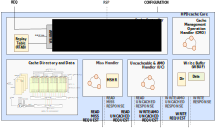
\includegraphics[width=\textwidth]{hpdcache_core.pdf}
  \caption{\figlabel{dcache_subsystem}HPDcache core}
\end{figure}

\section{Cache Controller}

The cache controller is responsible for decoding and issuing the requests to the appropriate handler.
The cache controller implements a 3-stage pipeline.
This pipeline is capable of accepting one request per cycle.
However, there are some scenarios where the pipeline, may either stall, or put a request on hold in a side buffer called \acf{RTAB}.

The first stage (stage 0) of the pipeline arbitrates between requests from the miss handler (refill), \ac{RTAB}, and requesters; the second stage (stage 1) responds to loads (in case of hit) and to stores; the third stage (stage 2) is only used by loads in case of miss.
In this last stage, the cache allocates a new entry in the \ac{MSHR}.

A request on stage 0 can either be consumed on that cycle (forwarded to the stage 1 or to the \ac{RTAB}), or wait, when the pipeline is stalled.
A request on stage 1 or stage 2 always advances.
In stage 1 the request is either acknowledged (load hit or write acknowledgement), forwarded to stage 2 (load miss), or put into the \ac{RTAB}.

\paragraph{Pipeline stalls in stage 0}\mbox{}

Stalls in stage 0 are necessary in some specific scenarios, that are listed below.
When there is a stall in stage 0, a new request from a requester cannot be accepted, this is, the corresponding $\mathsf{READY}$ signal is kept low (see \secref{if_valid_ready}).
Requests in the other stages (1 and 2) are processed normally (even in case of a stall in stage 0).

\begin{description}
\item[Event 1:] The \ac{RTAB} is full;
\item[Event 2:] A \ac{CMO} invalidation or fence operation is being processed by the corresponding handler;
\item[Event 3:] An uncacheable or atomic operation is being processed by the corresponding handler;
\item[Event 4:] There is a load miss in stage 1;
\item[Event 5:] There is a store in stage 1 and the request in stage 0 is a load (structural hazard on access to the internal cache data memory);
\end{description}

The number of clock cycles of the stall in stage 0 depends on the type of event:
\begin{itemize}
\item \textbf{Events~4~\&~5}: the number of clock cycles is always one.
\item \textbf{Events~1,~2~\&~3}: the number of clock cycles is variable:
  \begin{itemize}
  \item \textbf{Event~1}: it depends on when an entry of the \ac{RTAB} is freed.
  \item \textbf{Events~2~\&~3}: it depends on the latency of the corresponding operation.
  \end{itemize}
\end{itemize}


\subsection{On-Hold Requests}
\seclabel{onhold}

In some scenarios, a request that has been accepted in the pipeline can be later put on-hold by the cache controller.
When a request is put on-hold, it is re-executed when all the blocking conditions have been removed.
The blocking conditions putting a request on-hold are the following:

\begin{description}
  \item[Case 1:] \textbf{Cacheable LOAD or PREFETCH, and there is a hit on a pending miss (hit on the \acs{MSHR})}

When there is a read miss on an address (cacheline granurality) for which there is a pending read miss, then the more recent one needs to wait for the previous one to be served.
This allows the latest one to read the data from the cache after the refill operation completes.

  \item[Case 2:] \textbf{Cacheable LOAD or PREFETCH, there is a miss on the cache, and there is a hit (cacheline granularity) on an opened, closed or sent entry of the \ac{WBUF}}

When there is a read miss on an address, the cache controller needs to read from the memory the missing cacheline.
As the \ac{NoC} implements different physical channels for read and write requests, there is a race condition between the read miss and a pending write operation.
If the read miss arrives first to the memory, it would read the old data (which violates data consistency rules~\secref{rtab_mcr}).
This blocking condition causes that the LOAD or PREFETCH will have a delay penalty of up to two transaction delays: one for the write to complete, then one for the read.

  \item[Case 3:] \textbf{Cacheable STORE, there is a miss on the cache, and there is a hit on a pending miss (hit on the \acs{MSHR})}

When writing, as the \ac{NoC} implements different physical channels for read and write requests, there is a race condition between the STORE and the pending read miss.
If the STORE arrives first to the memory, the earlier read miss would read the new data (which violates data consistency rules in~\secref{rtab_mcr}).

  \item[Case 4:] \textbf{Cacheable STORE, and there is a hit on a closed entry of the \ac{WBUF}, or the \ac{WBUF} is full}

Writes on the same address need to be sent in order (to respect data consistency rules).
When there is a closed entry in the \ac{WBUF}, this means that it is waiting to be sent to the memory.
While it is not sent, the cache cannot open a new entry in the \ac{WBUF} for the same address, because they may be sent in an arbitrary order.

  \item[Case 5:] \textbf{Cacheable LOAD/PREFETCH/STORE, and there is a hit on an entry of the \ac{RTAB}}

Accesses to the same address (in cacheline granularity) MUST be processed in order (to respect data consistency rules).
In case of a hit with a valid entry in the \ac{RTAB}, the new request is written into the corresponding list of the \ac{RTAB}.

  \item[Case 6:] \textbf{Cacheable LOAD or PREFETCH, there is a miss on the cache, and the \acs{MSHR} has no available slots}

When there is a read miss on an address, the cache controller needs to allocate a new entry in the \acs{MSHR}.
The \acs{MSHR} is a set-associative memory.
If there is no available WAY to store the new read miss request, then this request needs to wait for an entry in the \ac{MSHR} with the corresponding SET to be freed.
This is when a refill operation is completed for a cacheline with the same \acs{MSHR} SET index.

  \item[Case 7:] \textbf{Cacheable LOAD or PREFETCH, there is a miss on the cache, and the miss handler FSM cannot send the read miss request}

When there is a read miss on an address, the cache controller needs to read from memory the missing cacheline.
The read miss request is sent by the miss handler FSM, but if there is congestion in the \ac{NoC}, this read request cannot be issued.
To avoid blocking the pipeline and creating a deadlock, the request is put on-hold.

\end{description}

All these conditions, except for case 5, are checked on the second stage (stage 1) of the pipeline.
Case 5 is checked in the first stage (stage 0) of the pipeline.
If one of the conditions is met, the request is put into the \ac{RTAB}.
It is kept on-hold until its blocking condition is solved.
At that moment, the request can be replayed from the \ac{RTAB} on the pipeline from stage 0.

The \ac{RTAB} can store multiple requests (on-hold requests).
The idea is to improve the throughput of the cache by reducing the number of cases where there is a head of line blocking at the client interface.

When a request cannot be processed right away, because it depends on the completion of a previous one, the request is stored in the replay table.
This allows new requests to arrive to the data cache and to be potentially executed (in an out-of-order fashion).
To prevent a deadlock, if the \ac{RTAB} is full, the \ac{HPDcache} does not accept new requests.

The ready requests in the \ac{RTAB} have higher priority than new requests.
These requests are executed as soon as possible, that is, when their dependencies are resolved.

To execute a request from the \ac{RTAB}, the cache controller complies to the rules defined in~\secref{rtab_mcr}.

\subsection{\acfp*{MCR}}%
\seclabel{rtab_mcr}

When multiple requests are put on-hold in the \ac{RTAB}, the cache controller may issue them (once they are ready) in a different order than the order in which they arrived (program order).
However, the cache controller needs to respect certain rules, here called \aclp{MCR}, to allow the requesters to have a predictable behavior.

The set of rules followed by the cache controller are those defined by the \ac{RVWMO} memory consistency model~\cite{RISCV_spec}.
A brief statement summarizing these rules is the following: \textbf{if one memory access (read or write), A, precedes another memory access (read or write), B, and they access overlapping addresses, then they MUST be executed in program order (A then B)}.
It can be deduced from this statement, that non-overlapping accesses can be executed in any order.

Of course, the cache controller also needs to respect the progress axiom: \textbf{"no memory operation may be preceded by an infinite number of memory operations"}.
That is, all memory operations need to be processed at some point in time, thus cannot wait indefinitely.


\section{Miss Handler}

This block is in charge of handling read miss requests to the memory.
It has three parts:
\begin{enumerate}
\item The first part is in charge of forwarding read miss requests to the memory;
\item The second part is in charge of tracking the status of in-flight read misses;
\item The third part is in charge of writing into the cache the response data from the memory, and update the cache directory accordingly.
\end{enumerate}

\Todo{Add FIFO buffer for storing miss requests to the MISS HANDLER.
This allows to reduce the number of requests put on-hold when the read request \ac{NoC} is congested.}


\subsection{Multiple-entry \acf*{MSHR}}
\seclabel{mshr}

The second part (tracking) of the miss handler contains an essential component of the \ac{HPDcache}: the set-associative multi-entry \ac{MSHR}.
Each entry of this component contains the status for each in-flight read miss request to the memory.
Therefore, the number of entries in the \ac{MSHR} defines the maximum number of in-flight read miss requests.

The number of entries in the \ac{MSHR} depends on two configuration values: $\mathsf{CONF\_DCACHE\_MSHR\_WAYS}$ and $\mathsf{CONF\_DCACHE\_MSHR\_SETS}$.
The number of entries is computed as:
\begin{equation*}
\mathsf{DCACHE\_MSHR\_SETS~\times~CONF\_DCACHE\_MSHR\_WAYS}
\end{equation*}

As for any set-associative array:

\begin{tabular}{p{\linewidth}}
    \toprule
    When $\mathsf{CONF\_DCACHE\_MSHR\_SETS = 1}~\text{and}~\mathsf{CONF\_DCACHE\_MSHR\_WAYS > 1}$\\
    $\rightarrow$~The \ac{MSHR} behaves as a fully-associative access array.\\
    \midrule
    When $\mathsf{CONF\_DCACHE\_MSHR\_SETS > 1}~\text{and}~\mathsf{CONF\_DCACHE\_MSHR\_WAYS = 1}$\\
    $\rightarrow$~The \ac{MSHR} behaves as a direct access array.\\
    \midrule
    When $\mathsf{CONF\_DCACHE\_MSHR\_SETS > 1}~\text{and}~\mathsf{CONF\_DCACHE\_MSHR\_WAYS > 1}$\\
    $\rightarrow$~The \ac{MSHR} behaves as a set-associative access array\\
\end{tabular}

A high number of entries in the \ac{MSHR} allows to overlap multiple accesses to the memory, and hides its latency.
Of course, the more entries there are, the more area the \ac{MSHR} consumes.
Therefore, the system architect must choose \ac{MSHR} parameters depending on a combination of memory latency, memory throughput, required area and performance, and the capability of requesters to issue multiple read transactions.

\begin{tcolorbox}[colback=red!10!white,
                  colframe=white!10!red,
                  title=\textbf{Important},
                  center, valign=top, halign=left,
                  center title,
                  width=.950\linewidth]
Regarding the last condition, regardless whether the requesters can issue multiple read requests, the hardware memory prefetcher exploits having multiple in-flight read miss requests.
\end{tcolorbox}

An entry in the \ac{MSHR} contains the following information:

\begin{center}
\begin{tabular}{lccccc}
\toprule%
{\bf Bits} &%
T &%
R &%
S &%
W &%
1 \\
\midrule
{\bf Description} &%
MSHR Tag &%
Request ID &%
Source ID &%
Word Index &%
Need Response\\
\end{tabular}

\begin{tabular}{ll}
\toprule%
{\bf Field} &%
{\bf Width} \\
\midrule%
MSHR tag (T) &%
$\mathsf{T = DCACHE\_NLINE\_WIDTH - log_2(CONF\_DCACHE\_MSHR\_SETS)}$ \\
\midrule%
Request ID (R) &%
$\mathsf{R = CONF\_DCACHE\_REQ\_TRANS\_ID\_WIDTH}$ \\
\midrule%
Source ID (S) &%
$\mathsf{S = CONF\_DCACHE\_REQ\_SRC\_ID\_WIDTH}$ \\
\midrule%
Word Index (W) &%
$\mathsf{W = log_2(CONF\_DCACHE\_CL\_WORDS})$ \\
\end{tabular}
\end{center}

\subsubsection{\acs*{MSHR} implementation}
\seclabel{mshr_implementation}

In order to limit the area cost of the \ac{MSHR}, it can be implemented using SRAM macros.
The depth of the macros is $\mathsf{CONF\_DCACHE\_MSHR\_SETS\_PER\_RAM}$.
Multiple ways, for the same set, can be put side-by-side in the same SRAM word ($\mathsf{CONF\_DCACHE\_MSHR\_WAYS\_PER\_RAM\_WORD}$), therefore the width is a multiple of $\mathsf{DCACHE\_MSHR\_ENTRY = T + R + S + W + 1}$ bits.
The total number of SRAM macros is:

\begin{equation*}
\begin{split}
\mathsf{(CONF\_DCACHE\_MSHR\_WAYS/CONF\_DCACHE\_MSHR\_WAYS\_PER\_RAM\_WORD)\times} \\
\mathsf{\lceil{}CONF\_DCACHE\_MSHR\_SETS/CONF\_DCACHE\_MSHR\_SETS\_PER\_RAM{}\rceil}
\end{split}
\end{equation*}

SRAM macros shall be selected depending on the required number of entries, and the target technology node. Additional information about \ac{MSHR} SRAM macros can be found in \apxref{ram_macros}.
When the number of entries is low (e.g. sets times ways are less than 16), it is generally better to implement the \ac{MSHR} using flip-flops.

This makes \ac{MSHR} fully-associative and thus removes associativity conflicts.


\section{Uncacheable Handler}

This block is responsible for handling uncacheable (see \secref{if_req_uncacheable}) load and store requests, as well as atomic requests (regardless of whether they are cacheable or not).
For more information about atomic requests see \charef{amo}.

All requests handled by this block produce a request to the memory.
This request to the memory is issued through the memory uncached interfaces.
Uncacheable read requests are forwarded to the memory through the memory read uncached interface (\tabref{if_mem_uc_read});
and uncacheable write requests or atomic requests are forwarded through the memory write uncached interface (\tabref{if_mem_uc_write}).


\section{\acf{CMO} Handler}

This block is responsible for handling \acp{CMO}.
\acp{CMO} are special requests from requesters that address the cache itself, and not the memory nor a peripheral.
These operations allow to either invalidate designated cachelines in the cache, or produce explicit memory read and write fences.

The complete list of supported \acp{CMO} is detailed in \charef{cmo}.

\section{Cache Directory and Data}

\subsection{RAM Organization}
\seclabel{dir_data_ram_implementation}

The \ac{HPDcache} cache uses RAM macros for the directory and data parts of the cache.
These RAM macros are synchronous, read/write, single-port RAMs.
Additional information about RAM macros in the cache can be found in \apxref{ram_macros}.

The organization of the RAMs, for the directory and the data, targets the following:
\begin{enumerate}[itemsep=1em]
\item {\bf High memory bandwidth to/from the requesters}

To improve performance, the organization allows to read one data word (1, 2, 4, 8, 16 or 32 bytes) per cycle, with a latency of one cycle.

\item {\bf Low energy-consumption}

To limit the energy-consumption, the RAMs are organized in a way that the cache enables only a limited number of RAM macros.
This number depends on the number of requested bytes, and it also depends on the target technology.
Depending on the target technology, the RAM macros have different trade-offs between width, depth and timing (performance).

\item {\bf Small RAM footprint}

To limit the footprint of RAMs, the selected organization implements a small number of RAMs macros.
The macros are selected in a way that they are as deep and as wide as possible.
The selected ratios (depth x width) depend on the target technology as explained above.

\end{enumerate}

\subsection{Example cache data/directory RAM organization}

\Figref{dcache_ram_organization} illustrates an example organization of the RAMs.
The illustrated organization allows to implement 32 KB of data cache (128 sets, 4 ways, and 64 bytes lines).
This example organization has a refilling latency of two cycles because the cache needs to write two different entries on a given memory cut.

\begin{figure}[htbp]
  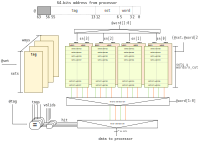
\includegraphics[width=\textwidth]{hpdcache_data_ram_organization.pdf}
  \caption{\figlabel{dcache_ram_organization}Data Cache Micro-Architecture}
\end{figure}

The example RAM organization in \figref{dcache_ram_organization} allows to access from 1 to 32 bytes of a given cacheline per cycle.

The energy consumption is dependent on the length of the access. Accesses from 1 to 8 bytes need to read two memory cuts (one containing ways 0 and 1, and the other containing ways 2 and 3); accesses from 8 to 16 bytes need to read 4 memory cuts; and so on. For reading 24 to 32 bytes, the cache needs to access all the cuts at the same time (8 cuts).

\section{\acf*{RTAB}}

The \ac{RTAB} is implemented as an array of linked lists.
It is a fully-associative multi-entry buffer, where each valid entry, belongs to a linked list.
It is implemented in flip-flops.
The linked lists contain a list of requests that target the same cacheline.
There can be multiple linked lists, but each shall target a different cacheline.
The head of each linked list contains the oldest request while the tail contains the newest request.
The requests are processed from the head to the tail in order to respect the \acp{MCR} explained in section \secref{rtab_mcr}.

Regarding the pop operation (extracting a ready request from the replay table), it is possible that once the request is replayed, some of the resources it needs are again busy.
Therefore, the request needs to be put on-hold again.
In this case, the request needs to keep its position as head of the linked list.
This is to preserve the program order.
For this reason, the pop operation is implemented as a two-step operation: pop then commit, or pop then rollback.
The commit operation allows to actually remove the request, while the rollback allows to undo the pop.

An entry of the \ac{RTAB} has the following structure (LL means Linked List):

\begin{center}
\begin{tabular}{p{.15\linewidth}p{.10\linewidth}p{.10\linewidth}p{.10\linewidth}p{.10\linewidth}p{.07\linewidth}}
  \toprule%
  Request \mbox{($\approx$200 bits)} & \mbox{LL tail} \mbox{(1 bit)} & \mbox{LL head} \mbox{(1 bit)} & \mbox{LL next} \mbox{(2-3 bits)} & Deps \mbox{(5 bits)} & Valid \mbox{(1 bit)} \\
  \midrule%
\end{tabular}
\end{center}

\begin{itemize}
\item Request: contains the on-hold request from the core (data + meta-data).
\item LL tail: indicates if the entry is the tail of a linked list.
\item LL head: indicates if the entry is the head of a linked list.
\item LL next: designates the next (older) request in the linked list.
\item Deps bits: indicates the kind of dependency that keeps the request on-hold.
\item Valid: indicates if the entry contains valid information (if unset the entry is free).
\end{itemize}

The following table briefly describes the possible dependencies between memory requests.
For each kind of dependency, there is a corresponding bit in the "deps bits" field of \ac{RTAB} entries.

\begin{tabular}{p{.30\linewidth}p{.70\linewidth}}
  \toprule%
  \bf Dependency
  & \bf Description \\
  \midrule%
  MSHR\_hit
  & There is an outstanding miss request on the target address \\
  \midrule%
  MSHR\_full
  & The MSHR is full \\
  \midrule%
  MISS\_handler\_busy
  & The MISS HANDLER is busy and cannot send a new miss request \\
  \midrule%
  WBUF\_hit
  & There is a match with a open, closed, or sent entry in the write buffer \\
  \midrule%
  WBUF\_not\_ready
  & There is a match with a closed entry in the write buffer or the write-buffer is full\\
\end{tabular}

\paragraph{\ac{RTAB} operations}\mbox{}

The \ac{RTAB} implements the following operations:

\begin{tabular}{p{.30\linewidth}p{.70\linewidth}}
  \toprule
  \textbf{Operation}                  & \textbf{Description} \\
  \midrule
  $\mathsf{rtab\_alloc()}$            & Allocate a new linked list \\
  \midrule
  $\mathsf{rtab\_alloc\_and\_link()}$ & Allocate a new entry and link it to an existing linked list \\
  \midrule
  $\mathsf{rtab\_pop\_try()}$         & Get a ready request from one of the linked list (wihout actually removing it from the list) \\
  \midrule
  $\mathsf{rtab\_pop\_commit()}$      & Actually remove a popped request from the list \\
  \midrule
  $\mathsf{rtab\_pop\_rollback()}$    & Rollback a previously popped request (with a possible update of its dependencies) \\
  \midrule
  $\mathsf{rtab\_find\_ready()}$      & Find a ready request among the heads of valid linked lists \\
  \midrule
  $\mathsf{rtab\_find\_empty()}$      & Find an empty request \\
  \midrule
  $\mathsf{rtab\_empty()}$            & Is the RTAB empty ? \\
  \midrule
  $\mathsf{rtab\_full()}$             & Is the RTAB full ? \\
  \midrule
  $\mathsf{update\_deps()}$           & Update the dependency bits of valid requests \\
\end{tabular}

\begin{lstlisting}[language=c]
int rtab_alloc(req_t r, deps_t d)
{
  int index = rtab_find_empty_entry();
  rtab[index] = {
    valid     : 1,
    deps      : d,
    ll_head   : 1,
    ll_tail   : 1,
    ll_next   : 0,
    request   : r
  };
  return index;
}
\end{lstlisting}

\begin{lstlisting}
int rtab_alloc_and_link(req_t r, int n)
{
  int index = rtab_find_empty_entry();

  //  replace the tail of the linked list
  rtab[n].ll_tail = 0;

  //  add the new request as the tail of the linked list
  rtab[index] = {
    valid     : 1,
    deps      : 0,
    ll_head   : 0,
    ll_tail   : 1,
    ll_next   : n,
    request   : r
  };

  return index;
}
\end{lstlisting}

\begin{lstlisting}
req_t rtab_pop_try(int &index)
{
  index = rtab_find_ready_entry();

  // Temporarily unset the head bit. This is to prevent the
  // request to be rescheduled.
  rtab[index].ll_head = 0;

  return rtab[index].request;
}
\end{lstlisting}

\begin{lstlisting}
void rtab_pop_commit(int index)
{
  //  Change the head of the popped linked list
  //  (look for a valid entry with the next field
  //  pointing to the popped entry)
  for (int i = 0; i < RTAB_NENTRIES; i++) {
    if (rtab[i].valid && (i != index) && (rtab[i].next == index) {
      rtab[i].ll_head = 1;
    }
  }

  rtab[index].valid = 0;
}
\end{lstlisting}

\begin{lstlisting}
void rtab_pop_rollback(int index, bitvector deps)
{
  rtab[index].ll_head = 1;
  rtab[index].deps    = deps;
}
\end{lstlisting}

\begin{lstlisting}
int rtab_find_ready_entry(int last)
{
  // choose a ready entry using a round-robin policy
  int i = (last + 1) % RTAB_NENTRIES;
  for (;;) {
    //  ready entry found
    if (rtab[i].valid && rtab[i].ll_head && (rtab[i].deps == 0))
      return i;

    //  there is no ready entry
    if (i == last)
      return -1;

    i = (i + 1) % RTAB_NENTRIES;
  }
}
\end{lstlisting}

\begin{lstlisting}
int rtab_find_empty_entry()
{
  for (int i = 0; i < RTAB_NENTRIES; i++)
    if (!rtab[i].valid)
      return i;

  return -1;
}
\end{lstlisting}

\begin{lstlisting}
bool rtab_is_full()
{
  return (rtab_find_empty_entry() == -1);
}
\end{lstlisting}

\begin{lstlisting}
int rtab_is_empty()
{
  for (int i = 0; i < RTAB_NENTRIES; i++)
    if (rtab[i].valid)
      return 0;

  return 1;
}
\end{lstlisting}

\subsection{\ac{RTAB} integration in the cache}

The data cache has a 3-stages pipeline.
The \ac{RTAB} will be used in stages 0 and 1 (st0 and st1).
The following table summarizes the actions performed on the \ac{RTAB}:

{\footnotesize%
\begin{tabular}{%
p{.12\linewidth}p{.17\linewidth}p{.11\linewidth}p{.11\linewidth}p{.11\linewidth}p{.11\linewidth}p{.11\linewidth}p{.11\linewidth}}
  \toprule%
  {\bf \mbox{New Request}}
  & {\bf Match @ in \ac{RTAB}}
  & {\bf Match @ in \ac{MSHR}}
  & {\bf Match @ in \ac{WBUF}}
  & {\bf Cache Miss AND \ac{MSHR} is full}
  & {\bf Cache Miss AND Miss Handler is not ready}
  & {\bf \ac{WBUF} is full} \\
  \midrule%
  LOAD
  & $\mathsf{alloc\_and\_link}$ (st0)
  & $\mathsf{alloc\_new}$ (st1)
  & $\mathsf{alloc\_new}$ (st1)
  & $\mathsf{alloc\_new}$ (st1)
  & $\mathsf{alloc\_new}$ (st1)
  & $\phi$ \\
  \midrule%
  STORE
  & $\mathsf{alloc\_and\_link}$ (st0)
  & $\mathsf{alloc\_new}$ (st1)
  & $\mathsf{alloc\_new}$ (st1) (if $\mathsf{wbuf\_entry}$ is closed)
  & $\phi$
  & $\phi$
  & $\mathsf{alloc\_new}$ (st1) \\
  \midrule%
\end{tabular}}

\subsection{Policy for taking new requests in the data cache}

With the \ac{RTAB}, the cache has three possible sources of requests:
\begin{enumerate}
\item Requesters (new requests);
\item the \ac{RTAB} (on-hold requests);
\item the miss handler (refill requests).
\end{enumerate}

The policy to choose the request is as follows:

\begin{lstlisting}
rtab_req = rtab_find_ready_entry();
if (rtab_is_full()) {
  new_req = rtab_req;
} else {
  new_req = (rtab_req != -1) ? rtab_req : core_req;
}

accepted_req = round_robin(new_req, refill_req);
\end{lstlisting}

To summarize: \ac{RTAB} ready requests have higher priority than core requests (this is to flush the pipeline as fast as possible).
However, if the \ac{RTAB} is full, the cache does not accept core requests because if they need to be put on-hold that could cause a deadlock.
Then, between the refill requests, the \ac{RTAB} or the core requests, the data cache applies a round-robin policy.

\subsection{Possible improvements for the \acs*{RTAB} integration}

\begin{itemize}
  \item Avoid introducing a NOP after an entry is replayed (popped).
  This is currently done to simplify the resolution of a concurrent \verb$alloc_and_link$ and \verb$pop_commit$ where the request being allocated depends on the one being popped.
\end{itemize}


\section{Write-buffer}

This cache implements a write-through policy.
In this policy, the write accesses from requesters are systematically transferred to the memory, regardless of whether the write access hits or misses in the \ac{HPDcache}.

To decouple the acknowledgement from the memory to the \ac{HPDcache}, and the acknowledgement from the \ac{HPDcache} to the requester, this \ac{HPDcache} implements a write-buffer.
The goal is to increase the performance: the requester does not wait the acknowledgement from the memory, which may suffer from a very high latency.
Additionally, to improve the bandwidth utilization of data channels in the \ac{NoC}, the write-buffer implements coalescing of write data.

The write-buffer implements two different parts: directory and data.
The directory enables tracking of active writes.
The data buffers are used to coalesce writes from the requester.
Entries in the data buffers are usually wider ($\mathsf{CONF\_DCACHE\_WBUF\_WORDS}$) than the data interface of requesters.
This is to enable the coalescing of multiple writes onto contiguous addresses.

A given entry in the directory of the write-buffer may be in four different states:

\begin{center}
\begin{tabular}{lp{.8\linewidth}}
\textbf{FREE}   & The entry is available. \\
\textbf{OPEN}   & The entry is currently used by a previous write access.
The entry accepts new write accesses (in the same address range) for coalescing. \\
\textbf{CLOSED} & The entry does not accept any new writes, and is waiting to be sent to the memory. \\
\textbf{SENT}   & The entry was forwarded to the memory, and is waiting for the acknowledgement. \\
\end{tabular}
\end{center}

\subsection{Memory Write Consistency Model}
\seclabel{wbuf_mcr}

The \ac{HPDcache} complies with the \ac{RVWMO} memory consistency model.
Regarding writes, in this consistency model, there are two important properties:

\begin{enumerate}

\item The order in which write accesses on different addresses are forwarded to memory MAY differ from the order they arrived from the requester (program order);

\item Writes onto the same address, MUST be visible in order. If there is a data written by a write A on address @x followed by an another write B on the same address, the data of A cannot be visible after the processing of B.

\end{enumerate}

The second property allows write coalescing if the hardware ensures that the last write persists.

The write-buffer exploits the first property.
Multiple "in-flight" writes are supported due to the multiple directory and data entries.
These writes can be forwarded to the memory in an order different than the program order.

To comply with the second property, the write-buffer does not accept a write when there is an address conflict with a \textbf{CLOSED}, or \textbf{SENT} entry.
In that case, the write is put on-hold following the policy described in \secref{onhold}.
The system may choose to relax the constraint of putting a write on-hold in case of an address conflict with a \textbf{SENT} entry.
This can be relaxed when the \ac{NoC} guaranties in-order delivery.
The runtime configuration bit~$\mathsf{cfig\_wbuf.S}$~(see \tabref{cfig_wbuf}) shall be deasserted to relax this dependency.

\Todo{We could slightly modify the behavior in the CLOSED state. The write-buffer coalesces writes in CLOSED states as these are not yet sent, and the data is still present the data buffer.}

\subsection{Functional Description}
\seclabel{wbuf_funcdesc}

When an entry of the write-buffer directory is in the \textbf{OPEN} or \textbf{CLOSED} states, there is an allocated data buffer, and it contains data that has not yet been sent to the memory.
When an entry of the write-buffer directory is in the \textbf{SENT} state, the corresponding data was transferred to the memory, thus the corresponding data buffer was freed.
A given entry in the write-buffer directory goes from \textbf{FREE} to \textbf{OPEN} state when a new write is accepted, and cannot be coalesced with another \textbf{OPEN} entry (e.g. not in the same address range).

A directory entry passes from \textbf{OPEN} to \textbf{CLOSED} after a given number of clock cycles.
This number of clock cycles depends on different runtime configurable values.
Each directory entry contains a life-time counter.
This counter starts at 0 when a new write is accepted (\textbf{FREE}->\textbf{OPEN}), and incremented each cycle while in \textbf{OPEN}.
When the counter reaches~$\mathsf{cfig\_wbuf.threshold}$~(see \tabref{cfig_wbuf}), the write-buffer directory entry goes to \textbf{CLOSED}.
Another runtime configurable bit, $\mathsf{cfig\_wbuf.R}$~(see \tabref{cfig_wbuf}), defines the behavior of an entry when a new write is coalesced into an \textbf{OPEN} entry.
If this last configuration bit is set, the life-time counter is reset to 0 when a new write is coalesced.
Otherwise, the counter keeps its value.

The life-time of a given write-buffer directory entry is longer than the life-time of a data entry.
A given directory entry is freed (\textbf{SENT}->\textbf{FREE}) when the write acknowledgement is received from the memory.
The number of cycles to get an acknowledgement from the memory may be significant and it is system-dependent.
Thus, to improve utilization of data buffers, the number of entries in the directory is generally greater than the number of data buffers.
However, there is a trade-off between area and performance because the area cost of data buffers is the most critical cost in the write-buffer.
The synthesis-time parameters $\mathsf{CONF\_DCACHE\_WBUF\_DIR\_ENTRIES}$ and $\mathsf{CONF\_DCACHE\_WBUF\_DATA\_ENTRIES}$ define the number of entries in the write-buffer directory and write-buffer data, respectively.

\Todo{Investigate an implementation of the data buffers in RAM.
At most, only one entry is written and read per cycle in the write buffer.
Thus an implementation with a 2-ports RAM could be more efficient.
Write masks (at least at byte granularity) in the RAM are necessary to allow the write coalescing}

\subsubsection{Memory Fences}

In multi-core systems, or more generally, in systems with multiple \acs{DMA}-capable devices, when synchronization is needed, it is necessary to implement memory fences from the software.
In the case of RISC-V, there is specific instructions for this (i.e. fence).

Fence instructions shall be forwarded to the cache to ensure ordering of writes. The fence will force the write-buffer to send all pending writes before accepting new ones.
This cache implements two ways of signalling a fence: sending a specific \ac{CMO} instruction from the core (described later on \charef{cmo}), or by asserting $\mathsf{wbuf\_flush\_i}$ pin (during one cycle).


\section{Cache-coherency}
\seclabel{cache_coherency}

The current version of the cache does not implement any hardware cache-coherency protocol.

In multi-core systems integrating this cache, cache-coherency needs to be enforced by the software. To this end, this cache provides cache invalidation instructions among the supported \acp{CMO}. These are described in \charef{cmo}. These can be used to solve the cache-obsolescence problem.

As the cache implements a write-through policy, there is no memory-obsolescence problem. This is because all writes are forwarded to the memory.


%\textit{Note: To solve the memory obsolescence problem using a write-back policy, we need to implement dirty bits in the cache directory.
%However, to support a byte granularity, we would need to implement 64 bits per cacheline, which represents an overhead of almost 13\% in the RAM area of the cache (considering a 32 KB cache).}

% \section{Write-back Data}

% The directory implements a given number of dirty bits per cacheline.
%Dirty bits indicate which data has been locally modified in the cache and therefore, the next levels of memory contain an obsolete state.
%In case of a cacheline eviction, only "dirty" data is actually write-back upstream.

% In the simplest case, L1 caches implement a single dirty bit.
%This means that anytime a modified cacheline needs to be evicted, even if a single bit has been modified, the entire cacheline is written-back.
%However, this behavior may cause problems when two different cores write in the same cacheline but different bytes (this situation is known as false-sharing).
%In that case, if no special mechanism is implemented, when a core writes-back a cacheline, it will potentially overwrite the changes from another core.
%When a write-invalidate cache-coherency protocol is implemented, this situation is avoided because a single core can own a modified cacheline.
%However, we do not implement a hardware cache-coherency protocol.

% In our case, to avoid the false-sharing problem we need a finer granularity for indicating the dirty data.
%One way is to have more than 1 dirty bit per cacheline.
%For example, we could implement 1-bit per 32-bits words.
%As we have 64 bytes cachelines, this would need 16 dirty bits per cacheline.

%\section{Cache Pipeline}

\clearpage
\chapter{\acfp{CSR}}
\chalabel{csr}
\minitoc
\newpage

\section{Dedicated CSR address space}
\seclabel{csr_address_space}

\begin{tcolorbox}[colback=red!10!white,
                  colframe=white!10!red,
                  title=\textbf{Important},
                  center, valign=top, halign=left,
                  center title,
                  width=.950\linewidth]
This CSR address space is not yet implemented in version 1.0.0 of the RTL.
In this version, runtime configuration values are passed through external ports of the HPDcache.
Performance counters are not implemented either.
\end{tcolorbox}

The \ac{HPDcache} defines a dedicated memory address space for configuring and checking the internal status.
This memory space is shared among all the requesters connected to the same \ac{HPDcache}.
However, this space is private to those requesters in a system-wide point of view.
This is, this dedicated \ac{CSR} address space is not visible to other requesters integrated in the system.

The dedicated \ac{CSR} address space is aligned to 4 Kibytes and has this same size.
Current version of the \ac{HPDcache} uses a very small subset of this address space, but the aligning to 4 Kibytes, allows easier mapping in the virtual address space by the \ac{OS}.
The smallest virtual/physical page size defined in the \citetitle{RISCV_privileged_spec}\cite{RISCV_privileged_spec} is 4 Kibytes.
This is the reason of this choice.
\Figref{csr_address_space} displays the layout of the dedicated \ac{CSR} address space of the \ac{HPDcache}.

The $\mathsf{CFIG\_BASE}$ address is specified through an input port of the \ac{HPDcache}.
The name of this input pin is \lstinline{cfig_base_i}.
It is a multi-bit signal.
The number of bits is $\mathsf{CONF\_DCACHE\_PA\_WIDTH}$.

\begin{figure}[!htbp]
\begin{center}
  \begin{tikzpicture}[scale=.7]
    \footnotesize
    \draw[line width=2] (0,0) rectangle (4,8);

    %  top line for segment 0
    \node at (2, 1) {\sf CFIG};
    \node [anchor=west] at (4, 0) {\sf CFIG\_BASE + 0x0000};
    \node [anchor=west] at (4, 2) {\sf CFIG\_BASE + 0x0200};
    \draw [line width=2](0,2)
      -- (4,2);

    %  top line for segment 1
    \node at (2, 3) {\sf CFIG\_HWPF};
    \node [anchor=west] at (4, 4) {\sf CFIG\_BASE + 0x0400};
    \draw [line width=2](0,4)
      -- (4,4);

    %  top line for segment 2
    \node at (2, 5) {\sf PERF};
    \node [anchor=west] at (4, 6) {\sf CFIG\_BASE + 0x0600};
    \draw [line width=2](0,6)
      -- (4,6);

    \node [anchor=west] at (4, 8) {\sf CFIG\_BASE + 0x800};
    \draw[fill=lightgray, draw=black, line width=2] (0,6) rectangle (4,8);
    \node [anchor=west] at (14, 8) {\sf CFIG\_BASE + 0x1000};
    \draw[fill=lightgray, draw=black, line width=2] (10,6) rectangle (14,8);
    \node [anchor=west] at (14, 6) {\sf CFIG\_BASE + 0xe00};
    \draw[fill=lightgray, draw=black, line width=2] (10,4) rectangle (14,6);
    \node [anchor=west] at (14, 4) {\sf CFIG\_BASE + 0xc00};
    \draw[fill=lightgray, draw=black, line width=2] (10,2) rectangle (14,4);
    \node [anchor=west] at (14, 2) {\sf CFIG\_BASE + 0xa00};
    \draw[fill=lightgray, draw=black, line width=2] (10,0) rectangle (14,2);
    \node [anchor=west] at (14, 0) {\sf CFIG\_BASE + 0x800};
  \end{tikzpicture}
  \caption{Dedicated CSR address space}%
  \figlabel{csr_address_space}
\end{center}
\end{figure}

\newpage
\section{Configuration registers}

\Tabref{csr_config} lists the configuration registers implemented in the \ac{HPDcache}.

These are mapped on the $\mathsf{CFIG}$ memory address segment in \figref{csr_address_space}.

\begin{figure}[!htbp]
  \begin{center}
    \caption{Configuration registers in the \ac*{HPDcache}}%
    \tablabel{csr_config}
    {\small%
    \begin{tabular}{p{.25\textwidth}p{.44\textwidth}p{.21\textwidth}}
      \textbf{CFIG Segment} & &\\
      \toprule
      \textbf{Register}
      & \textbf{Description}
      & \textbf{Base address} \\
      \toprule
      $\mathsf{cfig\_info}$
      & 64-bits register with cache information
      & $\mathtt{<CFIG\_BASE>~+~0x00}$\\
      \midrule
      $\mathsf{cfig\_ctrl}$
      & 64-bits register for configuring the cache controller
      & $\mathtt{<CFIG\_BASE>~+~0x08}$\\
      \midrule
      $\mathsf{cfig\_wbuf}$
      & 64-bits register for configuring the write-buffer
      & $\mathtt{<CFIG\_BASE>~+~0x10}$\\
      & & \\
      \textbf{CFIG\_HWPF Segment} & &\\
      \toprule
      \textbf{Register}
      & \textbf{Description}
      & \textbf{Base address} \\
      \toprule
      $\mathsf{cfig\_hwpf\_status}$
      & 64-bits register with the status of the hardware prefetcher
      & $\mathtt{<CFIG\_BASE>~+~0x200}$\\
      \midrule
      \verb$for (i = 0; i < 4; i++) {$ & & \\
      \midrule
      $\mathsf{cfig\_hwpf\_base\_engine[i]}$
      & 64-bits base cline register of the engine $\mathtt{i}$ of the hardware prefetcher
      & $\mathtt{<CFIG\_BASE>~+~0x200}$
        $\mathtt{+~(i~+~1)\times{}0x20~+~0x0}$\\
      \midrule
      $\mathsf{cfig\_hwpf\_param\_engine[i]}$
      & 64-bits parameters register of the engine $\mathtt{i}$ of the hardware prefetcher
      & $\mathtt{<CFIG\_BASE>~+~0x200}$
        $\mathtt{+~(i~+~1)\times{}0x20~+~0x8}$\\
      \midrule
      $\mathsf{cfig\_hwpf\_throttle\_engine[i]}$
      & 64-bits throttle register of the engine $\mathtt{i}$ of the hardware prefetcher
      & $\mathtt{<CFIG\_BASE>~+~0x200}$
        $\mathtt{+~(i~+~1)\times{}0x20~+~0x10}$\\
      \midrule
      \verb$}$ & & \\
      \bottomrule
    \end{tabular}}
  \end{center}
\end{figure}

\begin{minipage}{\textwidth}
\paragraph{$\mathbf{cfig\_info}$ - $\mathtt{<CFIG\_BASE>~+~0x00}$}\mbox{}\\[1em]
  \begin{bytefield}[endianness=big,bitwidth=\linewidth/64,%
    boxformatting={\centering\footnotesize\sf}]{64}
    \bitheader{0,7,8,15,16,19,20,23,48,63} \\
    \bitbox{16}{ID} &%
    \bitbox{24}{\color{lightgray}\rule{\width}{\height}} &%
    \bitbox{4}{HwPf} &%
    \bitbox{4}{LnSz} &%
    \bitbox{8}{Ways} &%
    \bitbox{8}{Sets}%
  \end{bytefield}

  \begin{center}
    {\footnotesize\begin{tabular}{p{.03\textwidth}p{.17\textwidth}p{.03\textwidth}p{.25\textwidth}p{.35\textwidth}}
    \textbf{Field} & \textbf{Description} & \textbf{Mode} & \textbf{Reset value}
    & \textbf{Comment}\\
    \toprule
    Sets & Number of sets & RO
    & $\mathsf{CONF\_DCACHE\_SETS}$
    & Indicates the number of sets implemented.\\
    \midrule
    Ways & Number of ways & RO
    & $\mathsf{CONF\_DCACHE\_WAYS}$
    & Indicates the number of ways implemented.\\
    \midrule
    LnSz & Number of bytes per cacheline (power of 2) & RO
    & $\mathsf{log_2(DCACHE\_CL\_WIDTH/8)}$
    & It contains the $\mathsf{log_2}$ of the size in bytes of cachelines.\\
    \midrule
    HwPf & Number of engines in the hardware prefetcher & RO
    & 4
    & Indicates the number of simultaneous streams supported by the hardware prefetcher \\
    \midrule
    ID & Version ID & RO
    & $\mathtt{0xCEA0}$
    & Version ID of the \ac{HPDcache}.\\
    \bottomrule
    \end{tabular}}
  \end{center}
\end{minipage}\\[1em]

\begin{minipage}{\textwidth}
\paragraph{$\mathbf{cfig\_ctrl}$ - $\mathtt{<CFIG\_BASE>~+~0x08}$}\mbox{}\\[1em]
  \begin{bytefield}[endianness=big,bitwidth=\linewidth/64,%
    boxformatting={\centering\footnotesize\sf}]{64}
    \bitheader{0,56,57,63} \\
    \bitbox{6}{\color{lightgray}\rule{\width}{\height}} &%
    \bitbox{1}{A} &%
    \bitbox{1}{R} &%
    \bitbox{55}{\color{lightgray}\rule{\width}{\height}} &%
    \bitbox{1}{E}%
  \end{bytefield}

  \begin{center}
    {\small\begin{tabular}{p{.05\textwidth}p{.30\textwidth}p{.05\textwidth}p{.05\textwidth}p{.40\textwidth}}
    \textbf{Field} & \textbf{Description} & \textbf{Mode} & \textbf{Reset value}
    & \textbf{Comment}\\
    \toprule
    E & Cache Enable & RW & \texttt{0b0}
    & When set to 0, all memory accesses are considered non-cacheable.\\
    \midrule
    R & Single-entry RTAB (fallback mode) & RW & \texttt{0b0}
    & This is a fallback mode. When set to 1, the cache controller only uses one entry in the \ac{RTAB}.\\
    \midrule
    A & Forbid AMO mode (\secref{amo_implementation}) & RW & \texttt{0b0}
    & When set to 1, the cache controller responds with an error to AMO requests targeting cacheable addresses.\\
    \bottomrule
    \end{tabular}}
  \end{center}
\end{minipage}\\[1em]

\begin{minipage}{\textwidth}
\paragraph{$\mathbf{cfig\_wbuf}$ - $\mathtt{<CFIG\_BASE>~+~0x10}$}\mbox{}\\[1em]
  \begin{bytefield}[endianness=big,bitwidth=\linewidth/64,%
    boxformatting={\centering\footnotesize\sf}]{64}
    \bitheader{0,1,8,15,63} \\
      \bitbox{48}{\color{lightgray}\rule{\width}{\height}} &%
      \bitbox{8}{Threshold}%
      \bitbox{6}{\color{lightgray}\rule{\width}{\height}} &%
      \bitbox{1}{S}%
      \bitbox{1}{R}%
  \end{bytefield}

  \begin{center}
    \tablabel{cfig_wbuf}
    {\small\begin{tabular}{p{.08\textwidth}p{.28\textwidth}p{.05\textwidth}p{.05\textwidth}p{.40\textwidth}}
    \textbf{Field} & \textbf{Description} & \textbf{Mode} & \textbf{Reset value}
    & \textbf{Comment}\\
    \toprule
    R & Reset time-counter on write & RW & \texttt{0b1}
    & When set to 1, writes restart the time-counter in the corresponding write-buffer entry.\\
    \midrule
    S & Sequential Write-After-Write & RW & \texttt{0b0}
    & When set to 1, the write-buffer holds-back writes requests that matches the target address of an on-the-fly write.\\
    \midrule
    Threshold & Number of keep-alive cycles of entries in the write-buffer & RW & \texttt{0x04}
    & The maximum accepted value is $\mathsf{CONF\_DCACHE\_WBUF\_TIMECNT\_MAX}$.
    When set to 0, a write immediatly closes the corresponding entry.\\
    \bottomrule
    \end{tabular}}
  \end{center}
\end{minipage}\\[1em]

\begin{minipage}{\textwidth}
\paragraph{$\mathbf{cfig\_hwpf\_*}$}\mbox{}\\[1em]
These registers are related to the hardware prefetcher.
They are mapped on the $\mathsf{CFIG\_HWPF}$ memory address segment.\\[1em]

Details on hardware prefetcher configuration registers are in \secref{prefetch_csrs}.
\end{minipage}\\[1em]


\section{Performance counters}
\seclabel{csr_performance}

The \ac{HPDcache} provides a set of performance counters.
These counters provide important information that can be used by software developers, at \ac{OS} level or user application level, to, for example, debug performance issues.

\Tabref{csr_performance} lists the performance counters provided by the \ac{HPDcache}.
These are mapped on the $\mathsf{PERF}$ memory address segment in \figref{csr_address_space}.

\begin{figure}[!htbp]
  \begin{center}
    \caption{Performance counters in the \ac*{HPDcache}}%
    \tablabel{csr_performance}
    {\footnotesize%
    \begin{tabular}{lll}
      \toprule
      \textbf{Counter}
      & \textbf{Description}
      & \textbf{Base address} \\
      \midrule
      $\mathsf{perf\_write\_req}$
      & 64-bits counter for processed write requests
      & $\mathtt{<PERF\_BASE>^\alpha~+~0x00}$\\
      \midrule
      $\mathsf{perf\_read\_req}$
      & 64-bits counter for processed read requests
      & $\mathtt{<PERF\_BASE>^\alpha~+~0x08}$\\
      \midrule
      $\mathsf{perf\_prefetch\_req}$
      & 64-bits counter for processed prefetch requests
      & $\mathtt{<PERF\_BASE>^\alpha~+~0x10}$\\
      \midrule
      $\mathsf{perf\_uncached\_req}$
      & 64-bits counter for processed uncached requests
      & $\mathtt{<PERF\_BASE>^\alpha~+~0x18}$\\
      \midrule
      $\mathsf{perf\_cmo\_req}$
      & 64-bits counter for processed \ac{CMO} requests
      & $\mathtt{<PERF\_BASE>^\alpha~+~0x20}$\\
      \midrule
      $\mathsf{perf\_accepted\_req}$
      & 64-bits counter for accepted requests
      & $\mathtt{<PERF\_BASE>^\alpha~+~0x28}$\\
      \midrule
      $\mathsf{perf\_cache\_write\_miss}$
      & 64-bits counter for write cache misses
      & $\mathtt{<PERF\_BASE>^\alpha~+~0x30}$\\
      \midrule
      $\mathsf{perf\_cache\_read\_miss}$
      & 64-bits counter for read cache misses
      & $\mathtt{<PERF\_BASE>^\alpha~+~0x38}$\\
      \midrule
      $\mathsf{perf\_on\_hold\_req}$
      & 64-bits counter for requests put on-hold
      & $\mathtt{<PERF\_BASE>^\alpha~+~0x40}$\\
      \bottomrule
      % empty
      & $\mathtt{\alpha:~<PERF\_BASE>~=~<CFIG\_BASE>~+~0x400}$
      &
    \end{tabular}}
  \end{center}
\end{figure}


\section{Event signals}
\seclabel{csr_events}

In addition to the performance registers explained in \secref{csr_performance}, the \ac{HPDcache} provides a set of one-shot signals that indicate when a given event is detected.
As one-shot signals, they are set to 1 for one cycle each time the corresponding event is detected.
If the same event is detected N cycles in a row, the corresponding event signal will remain set to 1 for N cycles.
\Tabref{csr_events} lists these event signals.

These event signals are output-only.
They can be either left unconnected, if they are not used, or connected with the remainder of the system.
The system can use those signals, for example, for counting those events externally or for triggering some specific actions.

\begin{figure}[!htbp]
  \begin{center}
    \caption{Event signals in the \ac*{HPDcache}}%
    \tablabel{csr_events}
    {\footnotesize%
    \begin{tabular}{ll}
      \toprule
      \textbf{Signal}
      & \textbf{Event description} \\
      \midrule
      $\mathsf{evt\_cache\_write\_miss\_o}$
      & Cache miss on write operation\\
      \midrule
      $\mathsf{evt\_cache\_read\_miss\_o}$
      & Cache miss on read operation\\
      \midrule
      $\mathsf{evt\_uncached\_req\_o}$
      & The cache processed an uncached request\\
      \midrule
      $\mathsf{evt\_cmo\_req\_o}$
      & The cache processed a \ac{CMO} request\\
      \midrule
      $\mathsf{evt\_write\_req\_o}$
      & The cache processed a write request\\
      \midrule
      $\mathsf{evt\_read\_req\_o}$
      & The cache processed a read request\\
      \midrule
      $\mathsf{evt\_prefetch\_req\_o}$
      & The cache processed a prefetch request\\
      \midrule
      $\mathsf{evt\_on\_hold\_req\_o}$
      & The cache put on-hold a request\\
      \bottomrule
  \end{tabular}}
  \end{center}
\end{figure}



\chapter{Cache Management Operations (CMOs)}
\chalabel{cmo}
\minitoc
\newpage

The \ac{HPDcache} is able of performing the following \aclp{CMO}:

\begin{itemize}
  \item memory write fence;
  \item invalidate a cacheline given a physical address;
  \item invalidate one or more cachelines in a given set given the set and one or more ways;
  \item invalidate all the cachelines;
  \item prefetch the cacheline indicated by its physical address.
\end{itemize}

Any of the clients of the DCACHE can trigger one of this operation anytime by using specific opcodes in their request.

\begin{table}[h!]
\begin{center}
\caption{CMO operation types}%
\tablabel{dcache_req_cmo}
{\footnotesize
\begin{tabular}{lll}
  \toprule
  \textbf{Mnemonic}
  & \textbf{Encoding}
  & \textbf{Type} \\
  \midrule
  $\mathsf{DCACHE\_CMO\_FENCE}$
  & 0b000
  & Memory write fence.\\
  \midrule
  $\mathsf{DCACHE\_CMO\_INVAL\_NLINE}$
  & 0b010
  & Invalidate a given cacheline.\\
  \midrule
  $\mathsf{DCACHE\_CMO\_INVAL\_SET\_WAY}$
  & 0b011
  & Invalidate one or more ways of in a given set of the cache.\\
  \midrule
  $\mathsf{DCACHE\_CMO\_INVAL\_ALL}$
  & 0b100
  & Invalidate the entire cache.\\
  \midrule
  $\mathsf{DCACHE\_CMO\_PREFETCH}$
  & 0b101
  & Prefetch a given cacheline.\\
  \midrule
\end{tabular}}
\end{center}
\end{table}

The $\mathsf{DCACHE\_REQ\_OP}$ must be set to $\mathsf{DCACHE\_REQ\_CMO}$ (see \tabref{dcache_req_op}).
The \ac{CMO} subtype (\tabref{dcache_req_cmo}) is transferred into the $\mathsf{DCACHE\_REQ\_SIZE}$ signal of the request.

The following sections describe in detail each of the \ac{CMO} operations, and how the requests shall be encoded to trigger each of them.


\newpage
\section{Memory write fence}

To make sure that the \ac{HPDcache} accepts new requests only when all previous writes are sent and acknowledged from the memory, a requester can issue a fence operation.

To do this, the requester shall build the request as follows:

{\centering\footnotesize\begin{tabular}{p{.38\linewidth}p{.55\linewidth}}
  \toprule
  \textbf{Signal}
  & \textbf{Value} \\
  \midrule
  $\mathsf{DCACHE\_REQ\_ADDR}$
  & *\\
  \midrule
  $\mathsf{DCACHE\_REQ\_OP}$
  & $\mathsf{DCACHE\_REQ\_CMO}$ \\
  \midrule
  $\mathsf{DCACHE\_REQ\_WDATA}$
  & *\\
  \midrule
  $\mathsf{DCACHE\_REQ\_BE}$
  & *\\
  \midrule
  $\mathsf{DCACHE\_REQ\_SIZE}$
  & $\mathsf{DCACHE\_CMO\_FENCE}$ \\
  \midrule
  $\mathsf{DCACHE\_REQ\_UNCACHEABLE}$
  & *\\
  \midrule
  $\mathsf{DCACHE\_REQ\_SID}$
  & Corresponding source ID of the requester\\
  \midrule
  $\mathsf{DCACHE\_REQ\_TID}$
  & Transaction identifier from the requester\\
  \midrule
  $\mathsf{DCACHE\_REQ\_NEED\_RSP}$
  & *\\
  \bottomrule
  & * means don't care \\
\end{tabular}}

As for any regular request, the request shall follow the \textbf{VALID}/\textbf{READY} handshake protocol described in \secref{if_valid_ready}.

This operation has the following effects:
\begin{itemize}
\item All open entries in the write buffer (write requests waiting to be sent to the memory) are immediately closed;
\item No new requests from any requester are acknowledged until all pending write requests in the cache have been acknowledged on the \ac{NoC} interface.
\end{itemize}


\newpage
\section{Invalidate a cacheline by its physical address}

To invalidate a cacheline by its physical address, the requester shall build the request as follows:

{\centering\footnotesize\begin{tabular}{p{.38\linewidth}p{.55\linewidth}}
  \toprule
  \textbf{Signal}
  & \textbf{Value} \\
  \midrule
  $\mathsf{DCACHE\_REQ\_ADDR}$
  & Physical address to invalidate in the cache.\\
  \midrule
  $\mathsf{DCACHE\_REQ\_OP}$
  & $\mathsf{DCACHE\_REQ\_CMO}$ \\
  \midrule
  $\mathsf{DCACHE\_REQ\_WDATA}$
  & *\\
  \midrule
  $\mathsf{DCACHE\_REQ\_BE}$
  & *\\
  \midrule
  $\mathsf{DCACHE\_REQ\_SIZE}$
  & $\mathsf{DCACHE\_CMO\_INVAL\_NLINE}$ \\
  \midrule
  $\mathsf{DCACHE\_REQ\_UNCACHEABLE}$
  & *\\
  \midrule
  $\mathsf{DCACHE\_REQ\_SID}$
  & Corresponding source ID of the requester\\
  \midrule
  $\mathsf{DCACHE\_REQ\_TID}$
  & Transaction identifier from the requester\\
  \midrule
  $\mathsf{DCACHE\_REQ\_NEED\_RSP}$
  & *\\
  \bottomrule
  & * means don't care \\
\end{tabular}}

As for any regular request, the request shall follow the \textbf{VALID}/\textbf{READY} handshake protocol described in \secref{if_valid_ready}.

For the sake of design simplification, this operation works as a memory read fence.
That is, before handling the operation, the \ac{HPDcache} waits for all pending read misses to complete.
Future versions of the HPDcache could wait only for a pending read miss on the same address that is being invalidated.

If the given physical address is not cached, the operation does nothing.
However it still works as a memory read fence.

Regarding the latency of this operation, it depends on the time to serve all pending read misses.
Only one cycle is needed to invalidate the corresponding cacheline.


\newpage
\section{Invalidate a group of cachelines by their a set and way}

To invalidate a group of cachelines, the requester shall build the request as follows:

{\centering\footnotesize\begin{tabular}{p{.38\linewidth}p{.55\linewidth}}
  \toprule
  \textbf{Signal}
  & \textbf{Value} \\
  \midrule
  $\mathsf{DCACHE\_REQ\_ADDR}$
  & Index of the set to invalidate.\\
  \midrule
  $\mathsf{DCACHE\_REQ\_OP}$
  & $\mathsf{DCACHE\_REQ\_CMO}$ \\
  \midrule
  $\mathsf{DCACHE\_REQ\_WDATA}$
  & Bit-vector with target ways to invalidate.
  The number of bits decoded depends on the number of ways implemented ($\mathsf{CONF\_DCACHE\_WAYS}$).
  The least significant bit corresponds to way 0, the second to way 1, etc.\\
  \midrule
  $\mathsf{DCACHE\_REQ\_BE}$
  & *\\
  \midrule
  $\mathsf{DCACHE\_REQ\_SIZE}$
  & $\mathsf{DCACHE\_CMO\_INVAL\_SET\_WAY}$\\
  \midrule
  $\mathsf{DCACHE\_REQ\_UNCACHEABLE}$
  & *\\
  \midrule
  $\mathsf{DCACHE\_REQ\_SID}$
  & Corresponding source ID of the requester\\
  \midrule
  $\mathsf{DCACHE\_REQ\_TID}$
  & Transaction identifier from the requester\\
  \midrule
  $\mathsf{DCACHE\_REQ\_NEED\_RSP}$
  & *\\
  \bottomrule
  & * means don't care \\
\end{tabular}}

As for any regular request, the request shall follow the \textbf{VALID}/\textbf{READY} handshake protocol described in \secref{if_valid_ready}.

For the sake of design simplification, this operation works as a memory read fence.
That is, before handling the operation, the \ac{HPDcache} waits for all pending read misses to complete.
Future versions of the HPDcache could wait only for a pending read misses on the same set that is being invalidated.

If the given set and ways contains no valid cachelines, the operation does nothing.
However it still works as a memory read fence.

Regarding the latency of this operation, it depends on the time to serve all pending reads.
Only one cycle is needed to invalidate the given set and ways because the ways are invalidated simultaneously.


\newpage
\section{Invalidate the entire cache}

With this operation, all the cachelines in the \ac{HPDcache} are invalidated.

To perform a complete invalidation of the \ac{HPDcache}, the requester shall build the request as follows:

{\centering\footnotesize\begin{tabular}{p{.38\linewidth}p{.55\linewidth}}
  \toprule
  \textbf{Signal}
  & \textbf{Value} \\
  \midrule
  $\mathsf{DCACHE\_REQ\_ADDR}$
  & *\\
  \midrule
  $\mathsf{DCACHE\_REQ\_OP}$
  & $\mathsf{DCACHE\_REQ\_CMO}$ \\
  \midrule
  $\mathsf{DCACHE\_REQ\_WDATA}$
  & *\\
  \midrule
  $\mathsf{DCACHE\_REQ\_BE}$
  & *\\
  \midrule
  $\mathsf{DCACHE\_REQ\_SIZE}$
  & $\mathsf{DCACHE\_CMO\_INVAL\_ALL}$\\
  \midrule
  $\mathsf{DCACHE\_REQ\_UNCACHEABLE}$
  & *\\
  \midrule
  $\mathsf{DCACHE\_REQ\_SID}$
  & Corresponding source ID of the requester\\
  \midrule
  $\mathsf{DCACHE\_REQ\_TID}$
  & Transaction identifier from the requester\\
  \midrule
  $\mathsf{DCACHE\_REQ\_NEED\_RSP}$
  & *\\
  \bottomrule
  & * means don't care \\
\end{tabular}}

As for any regular request, the request shall follow the \textbf{VALID}/\textbf{READY} handshake protocol described in \secref{if_valid_ready}.

This operation works as a memory read fence.
This is, before handling the operation, the \ac{HPDcache} waits for all pending read misses to complete.

Regarding the latency of this operation, it has two aggregated components:

\begin{itemize}
\item The time to serve all pending reads.
\item One cycle per set implemented in the \ac{HPDcache} (all ways of a given set are invalidated in simultaneously).
\end{itemize}


\newpage
\section{Prefetch a cacheline given its physical address}

With this operation, the cacheline corresponding to the indicated physical address is (pre-)fetched into the \ac{HPDcache}

To perform a prefetch, the requester shall build the request as follows:

{\centering\footnotesize\begin{tabular}{p{.38\linewidth}p{.55\linewidth}}
  \toprule
  \textbf{Signal}
  & \textbf{Value} \\
  \midrule
  $\mathsf{DCACHE\_REQ\_ADDR}$
  & *\\
  \midrule
  $\mathsf{DCACHE\_REQ\_OP}$
  & $\mathsf{DCACHE\_REQ\_CMO}$ \\
  \midrule
  $\mathsf{DCACHE\_REQ\_WDATA}$
  & *\\
  \midrule
  $\mathsf{DCACHE\_REQ\_BE}$
  & *\\
  \midrule
  $\mathsf{DCACHE\_REQ\_SIZE}$
  & $\mathsf{DCACHE\_CMO\_PREFETCH}$\\
  \midrule
  $\mathsf{DCACHE\_REQ\_UNCACHEABLE}$
  & *\\
  \midrule
  $\mathsf{DCACHE\_REQ\_SID}$
  & Corresponding source ID of the requester\\
  \midrule
  $\mathsf{DCACHE\_REQ\_TID}$
  & Transaction identifier from the requester\\
  \midrule
  $\mathsf{DCACHE\_REQ\_NEED\_RSP}$
  & Indicates if the requester needs an acknowledgement when the prefetch of the cacheline is completed.\\
  \bottomrule
  & * means don't care \\
\end{tabular}}

As for any regular request, the request shall follow the \textbf{VALID}/\textbf{READY} handshake protocol described in \secref{if_valid_ready}.

If the requested cacheline is already in the cache, at the moment the request is processed, this request has no effect. If the requested cacheline is not present in the cache, the cacheline is fetched from the memory and replicated into the cache.

When the prefetch transaction is completed, and the $\mathsf{DCACHE\_REQ\_NEED\_RSP}$ signal was set to 1, an acknowledgement is sent to the corresponding requester.


\chapter{Atomic Memory Operations (AMOs)}
\chalabel{amo}
\minitoc
\newpage

\section{Background}

The \acp{AMO} are special load/store accesses that implements a read-modify-write semantic.
A single instruction is able to read a data from the memory, perform an arithmetical/logical operation on that data, and store the result.
All this is performed as a single operation (no other operation can come in between the read-modify-write operations).

These operations are meant for synchronization in multi-core environments.
To enable this synchronization, \acp{AMO} need to be performed on the \acf{PoS}, point where all accesses from the different cores converge.
This is usually a shared cache memory (when multiple levels of cache are implemented) or the external RAM controllers.
Thus, the \ac{HPDcache} needs to forward these operations to the \ac{PoS} through the \ac{NoC} interface.

\section{Supported \acp*{AMO}}

On the interface from requesters, the supported \acp{AMO} are the ones listed in \tabref{dcache_req_op}.
The supported \acp{AMO} are the ones defined in the atomic (A) extension of the RISC-V ISA specification: \citetitle{RISCV_spec}\cite{RISCV_spec}.


\section{Implementation}
\seclabel{amo_implementation}

This cache does not implement a hardware cache-coherency protocol.
Therefore, the software needs to solve the cache obsolescence problem to ensure it reads the last value of the shared data.
There are two common ways of doing this:
\begin{enumerate}
\item Statically, by placing all shared data into uncacheable segments (never replicated in the \ac{HPDcache});

\item Dynamically, by explicitly invalidating local copies of shared data from the \ac{HPDcache}.
\end{enumerate}

The cache obsolescence problem applies to \acp{AMO}.
As these operations are used for implementing synchronization mechanism, the manipulated data is by nature shared and need to be coherent between the different caches.
The \ac{HPDcache} implements two different modes for handling \acp{AMO}:

\begin{description}
\item[Replicated AMO mode] \mbox{}\\%
Forward the \ac{AMO} to the \ac{PoS}, and wait for the response with the old data.
If the data of the target address is replicated in the \ac{HPDcache}, the \ac{HPDcache} computes the new value locally, and updates the target word in the corresponding cacheline.
With this solution the modified word with the \ac{AMO} will be up to date (coherent) with respect to the value in memory.
This solution needs explicit treatment from the software.
In particular, it requires that synchronization variables are always written (and possibly read) using \acp{AMO}.
For reading a shared variable, the software has two possibilities: (1) send an \ac{AMO} that does not modify the memory (e.g. AMOOR with bit-mask equal to zero); (2) invalidate the local cacheline prior to issuing the load instruction.

\item[Forbid AMO mode] \mbox{}\\%
This is a much more strict policy.
\acp{AMO} can only be performed on uncacheable memory addresses.
If requests do not follow this rule, an exception is signalled from the cache to the corresponding requester.

\end{description}

The \ac{HPDcache} supports both modes, but only one can be active at any given time.
The \verb$cfig_error_on_cacheable_amo$ configuration bit selects the mode of operation.
When this bit is set to 0, the \textbf{Replicated AMO mode} is active.
When this bit is set to 1, the \textbf{Forbid AMO mode} is active.

The \ac{HPDcache} handle \acp{AMO} as non-allocating operations, regardless of the \ac{AMO} mode described above.
This is, \acp{AMO} never fetch a replica of the target cacheline from the memory to the cache.
If the target cacheline IS NOT replicated in the cache, the \ac{AMO} modifies the memory.
If the target cacheline IS replicated in the cache, the \ac{AMO} modifies both the memory and the cache.

\section{AMO ordering}

As specified in the RISC-V ISA specification~\cite{RISCV_spec}, the base RISC-V ISA has a relaxed memory model.
To provide additional ordering constraints, \acp{AMO} (including \acs*{LR}/\acs*{SC}) specify two bits, \textit{aq} and \textit{rl}, for \textit{acquire} and \textit{release} semantics.

The \ac{HPDcache} always ignores \textit{aq} and \textit{rl} bits.
It considers that they are always set.
Hence, \ac{HPDcache} handles \acp{AMO} always as sequentially consistent memory operations.
The \ac{HPDcache} waits for all pending read and write operations to complete before serving the \ac{AMO} request.

This behavior implies that when the \ac{HPDcache} forwards an \ac{AMO} to the \ac{NoC}, it will be the only pending request from the \ac{HPDcache}.
In addition, no new requests from the requesters are served until the \ac{AMO} is completed.


\section{LR/SC support}

\acf{LR} and \acf{SC} are part of the Atomic (A) extension of the RISC-V ISA specification~\cite{RISCV_spec}.
These instructions allow {\it "complex atomic operations on a single memory word or double-word"}.

The \ac{HPDcache} fully supports all the instructions of the A extension of the RISC-V ISA, including \ac{LR} and \ac{SC} operations.

In the specification of these instructions in the RISC-V ISA document, some details are dependent to the implementation.
Namely, the size of the reservation set and the return code of a \ac{SC} failure.


\subsection{LR/SC reservation set}

When a requester executes a \ac{LR} operation, it "reserves" a set of bytes in memory.
This set contains at least the bytes solicited in the request but may contain more.
RISC-V ISA defines two sizes for \ac{LR} operations: 4 bytes or 8 bytes.
{\bf The \ac{HPDcache} reserves 8-bytes (double-word) containing the addressed memory location regardless of whether the \ac{LR} size is 4 or 8 bytes}.
The start address of the reservation set is a 8-bytes aligned address.

When the \ac{LR} size is 8 bytes, the address is also aligned to 8 bytes (\secref{if_addr_data_alignment}).
In this case, the reservation set matches exactly the address interval defined in the request.
When the \ac{LR} size is 4 bytes, there are two possibilities: (1)~the target address is not aligned to 8 bytes.
The start address of the reservation set contains additional 4 bytes before the target address ;
(2)~the target address is aligned to 8 bytes.
The reservation set starts at the target address but contains additional 4 bytes after the requested ones.

In summary, in case of \ac{LR} operation, the reservation set address range is computed as follows:

\begin{equation*}
    \mathbf{reservation\_set =}
    \begin{cases}
    \mathsf{\lfloor{}DCACHE\_REQ\_ADDR / 8\rfloor{} \times 8} &
      (start\_address) \\
    \mathsf{(\lfloor{}DCACHE\_REQ\_ADDR / 8\rfloor{} \times 8) + 8} &
      (end\_address) \\
    \end{cases}
\end{equation*}

{\bf When a requester executes a \ac{SC} operation, the \ac{HPDcache} forwards the operation to the memory ONLY IF the bytes addressed by the \ac{SC} are part of an active reservation set}.
If the \ac{SC} accesses a smaller number of bytes that those in the active reservation set but within that reservation set, the \ac{SC} is still forwarded to the memory.

The \ac{HPDcache} keeps an unique active reservation set.
If multiple requesters perform \ac{LR} operations, the unique active reservation set is the one specified by the last \ac{LR} operation.

\Todo{Could this be a problem ? Should we keep one reservation set per requester ?}

After a \ac{SC} operation, the unique active reservation set, if any, is invalidated.
This is regardless whether the \ac{SC} operation succeeds or not.


\subsection{\ac*{SC} failure response code}
\seclabel{sc_failure_code}

The RISC-V ISA~\cite{RISCV_spec} specifies that when a \ac{SC} operation succeeds, the core shall write zero into the destination register of the operation.
Otherwise, in case of \ac{SC} failure, the core shall write a non-zero value into the destination register.

The \ac{HPDcache} returns the status of an \ac{SC} operation into the $\mathsf{DCACHE\_RSP\_RDATA}$~(\tabref{if_rsp}) signal of the response interface to requesters.
The following table specifies the values returned by the \ac{HPDcache} into the $\mathsf{DCACHE\_RSP\_RDATA}$ signal in case of \ac{SC} operation.

\begin{center}
  {\small%
    \begin{tabular}{p{.15\linewidth}p{.20\linewidth}}
    \toprule
    \textbf{Case}
    & \textbf{Return value (status)}\\
    \midrule
    SC success
    & \texttt{0x0000\_0000} \\
    \midrule
    SC failure
    & \texttt{0x0000\_0001} \\
    \bottomrule
  \end{tabular}}
\end{center}

Depending on the specified size ($\mathsf{DCACHE\_REQ\_SIZE}$) in the request (\tabref{if_rsp}), the returned value is extended with zeros on the most significant bits.
This is, if the SC request size is 8 bytes, and the SC is a failure, then the returned value is \texttt{0x0000\_0000\_0000\_0001}.

In addition, if the width of the $\mathsf{DCACHE\_RSP\_RDATA}$ signal is wider than the size of the SC request, the return value is replicated $\mathsf{CONF\_DCACHE\_REQ\_WORDS}$~(\tabref{dcache_parameters}) times.


\chapter{Hardware Memory Prefetcher}
\minitoc
\newpage

In order to predict future data accesses and reduce the data cache miss rate, the cache implements a programmable hardware mechanism allowing to prefetch cachelines before they are actually requested.

The \ac{HPDcache} implements a prefetcher that contains multiple prefetch engines.
Each prefetch engine works independently, and simultaneously.
A round-robin arbiter at the output of the prefetcher allows to select one prefetch request from one of the engines per cycle.
This arbiter guarantees the correct behavior when multiple prefetch engines are active.

Each engine, if activated, fetches a stream of cachelines.
A stream is defined as a sequence of prefetch requests.
An engine reads one or multiple blocks of a given number of cachelines.
The first block starts at a given base cacheline.
Between blocks, one can configure a given address offset (also known as the stride).

The four parameters (base cacheline, number of cachelines in a block, number of blocks, and the stride) of each stream (one per engine) are configured through dedicated \acp{CSR}.

\section{Triggering}

A given prefetcher engine starts operating when the following conditions are met:

\begin{enumerate}
\item Each engine implements an enable bit in its dedicated \acp{CSR}.
This enable bit shall be set to 1 to allow the triggering of a given prefetcher engine.

\item Each enabled engine (condition 1 is met), snoops on the requests ports from the requesters.
If there is a match between the issued address and the configured base cacheline of the engine, the engine starts the prefetching.

\end{enumerate}

Once an engine starts its operation, it does not snoop anymore the request ports.
At that moment, it issues a sequence of prefetch operations starting from $\mathsf{base\_cline}$, until the cacheline in the equation below.
When the last cacheline is reached, the behavior of the engine is described in the following section.

\begin{equation*}
    \mathsf{end\_cline = base\_cline + (Nblocks + 1)\times{}(Stride + 1)}
\end{equation*}

A prefetch operation behaves as a read in the cache, but no data is expected in response by the prefetcher.
This means, that prefetch operations do not need to enable the data array of the cache (thus reducing the energy consumption for this operation).
Prefetch operations only access cache directory memories to check if the requested cacheline is cached or if it needs to be fetched from the memory.

\begin{tcolorbox}[colbacktitle=green!50!black,
                  colback=green!10!white,
                  colframe=green!50!black,
                  title=\textbf{Programming note},
                  center, valign=top, halign=justify,
                  center title,
                  width=.950\linewidth]

As explained in this section, a requester needs to issue a load transaction within the base cacheline of an engine to start its operation.

When the requester is a programmable processor core, an additional feature that could be implemented in the core is a software prefetch instruction.
This instruction would allow the software to prefetch a given cacheline, without stalling the core while waiting the response from the cache.
Such instruction could also be used to start an enabled prefetcher engine.

In RISC-V cores, one possibility to implement this software prefetch instruction could be to use the following:

\vspace{.8em}

\begin{verbatim}
lw x0, offset(rs1)
\end{verbatim}

\vspace{.8em}

As the \verb|x0| register is always equal to zero, the data is dropped.
Therefore, an efficient implementation of this instruction in the core consists on forwarding the load to the L1 data cache but do not wait for the response.
\end{tcolorbox}

\section{Activation/Deactivation Policies}
\seclabel{prefetch_activation_policies}

The prefetcher engines implement different automatic activation/deactivation policies:

\begin{tabular}{p{.3\linewidth}p{.65\linewidth}}
\toprule
\textbf{Policies}
& \\
\midrule
\textbf{Disarm when finished}
& When the engine completes the configured stream, it is automatically disabled.\\
\midrule

\textbf{Rearm when finished}
& When the prefetcher completes the configured stream, it does not disable.
However, it stops and waits to be triggered again.

At that point, the base cacheline \ac{CSR} of the engine saves the last accessed cacheline plus the stride.
This is, it saves the next address to prefetch.

The \acp{CSR} for the number of blocks, cachelines per block and stride keep their originally configured values.\\
\midrule

\textbf{Rearm and Cycle when finished}
& In this policy, the prefetch engine behaves as in the "Rearm when finished" policy, but the base cacheline \ac{CSR} is reset to the originally configured value.\\

\end{tabular}

\section{CSRs}
\seclabel{prefetch_csrs}

Each prefetcher engine has three dedicated \acp{CSR}.

\begin{itemize}
    \item Base cline (base cacheline) - $\mathsf{cfig\_hwpf\_base\_engine}$~(see \tabref{csr_config})

    \begin{bytefield}[endianness=big,bitwidth=\linewidth/64,%
      boxformatting={\centering\footnotesize\sf}]{64}
      \bitheader{0,1,2,3,4,5,6,63} \\
        \bitbox{58}{Base~cline} &%
        \bitbox{2}{\color{lightgray}\rule{\width}{\height}} &%
        \bitbox{1}{U} &%
        \bitbox{1}{C} &%
        \bitbox{1}{R} &%
        \bitbox{1}{E}%
    \end{bytefield}

    \begin{tabular}{ll}
      \textbf{E:} & Enable bit \\
      \textbf{R:} & Rearm bit \\
      \textbf{C:} & Cycle bit \\
      \textbf{U:} & Upstream bit \\
    \end{tabular}

    \begin{tabular}{lll}
      \textbf{Mode}                  & \textbf{R} & \textbf{C} \\
      Disarm when finished           & 0          & X \\
      Rearm when finished            & 1          & 0 \\
      Cycle and rearm when finished  & 1          & 1 \\
    \end{tabular}

  \item Parameters - $\mathsf{cfig\_hwpf\_param\_engine}$~(see \tabref{csr_config})

    \begin{bytefield}[endianness=big,bitwidth=\linewidth/32,%
      boxformatting={\centering\footnotesize\sf}]{32}
      \bitheader[lsb=32]{32,47,48,63} \\
        \bitbox{16}{Nblocks} &%
        \bitbox{16}{Nlines} &%
        \\[.5em]%
      \bitheader[lsb=0]{0,31} \\
        \bitbox{32}{Stride} &%
    \end{bytefield}

  \item Throttle - $\mathsf{cfig\_hwpf\_throttle\_engine}$~(see \tabref{csr_config})

    \begin{bytefield}[endianness=big,bitwidth=\linewidth/32,%
      boxformatting={\centering\footnotesize\sf}]{32}
      \bitheader[lsb=0]{0,15,16,31} \\
        \bitbox{16}{Ninflight} &%
        \bitbox{16}{Nwait} &%
    \end{bytefield}
\end{itemize}

\begin{description}

\item [\textsf{Stride} parameter] \mbox{}\\
It is an unsigned, one-based ($\mathsf{value + 1}$), 32-bits wide value.
The stride is in number of cachelines.
This means that the stride is always a multiple of $\mathsf{(DCACHE\_CL\_WIDTH/8)}$ bytes.

\item [\textsf{Nblocks} parameter] \mbox{}\\
It is an unsigned, one-based ($\mathsf{value + 1}$), 16-bits wide value.
This value corresponds to the number of blocks to prefetch.
The 16-bit value allows the prefetcher to prefetch up to 65536 blocks (of at least one cacheline).
This parameter is clearly over-dimensioned with respect to the usual capacity of the \ac{HPDcache} (e.g. 512, 64-byte, cachelines with a 32KB capacity).

\item [\textsf{Nlines} parameter] \mbox{}\\
It is an unsigned, one-based, 16-bits wide value.
It indicates the number of cachelines within blocks.
As the number of bits is 16, the maximum number of cachelines in a given block is 65536.

\item [\textsf{Nwait} parameter] \mbox{}\\
It is an unsigned, one-based, 16-bits wide value.
It defines the number of cycles (plus 1) between two requests of the prefetcher engine.
The zero value indicates that the engine can issue a request every cycle.

\item [\textsf{Ninflight} parameter] \mbox{}\\
It is an unsigned, zero-based, 16-bits wide value.
It defines the maximum number of in-flight (sent but not yet acknowledged) transactions from the prefetcher engine.
This parameter allows to throttle the memory bandwidth solicited by the prefetcher engine.
The zero value indicates that the number of in-flight transactions is unlimited.

\item [\textsf{U} bit] \mbox{}\\
When this upstream bit is set, prefetch operations targets the next level in the memory hierarchy.
In this case, upstream prefetch operations do not allocate cachelines in the L1 data-cache.
These are forwarded to the next memory level that can then prefetch the requested address.
THIS BIT IS NOT CURRENTLY IMPLEMENTED AND IGNORED.

\item [\textsf{C} bit] \mbox{}\\
This bit is only considered when the R bit (rearm) is also set.
When this cycle bit is set, after the prefetcher engine completes the prefetch stream, it resets the base cacheline to the originally configured one (see \secref{prefetch_activation_policies}).

\item [\textsf{R} bit] \mbox{}\\
When this rearm bit is set, after the prefetcher engine completes the prefetch stream, it "rearms" itself (remains enabled), and snoops for core requests (see \secref{prefetch_activation_policies}).
The address it snoops after it finishes depends on the Cycles (C) bit.
If the C bit is set, the behavior is described here above.
If the C bit is unset, after the prefetcher engine finishes, the snoop address is set to $\mathsf{end\_cline}$.

\end{description}

There is also a global status register for the prefetcher to monitor the status of the different prefetcher engines:

\begin{itemize}
  \item Status register

    \begin{bytefield}[endianness=big,bitwidth=\linewidth/16,%
      boxformatting={\centering\footnotesize\sf}]{16}
      \bitheader[lsb=48]{48,63} \\
        \bitbox{16}{\color{lightgray}\rule{\width}{\height}} &%
        \\[.5em]%
      \bitheader[lsb=32]{32,33,34,35,36,47} \\
        \bitbox{12}{\color{lightgray}\rule{\width}{\height}} &%
        \bitbox{1}{P3 busy} &%
        \bitbox{1}{P2 busy} &%
        \bitbox{1}{P1 busy} &%
        \bitbox{1}{P0 busy}%
        \\[.5em]%
      \bitheader[lsb=16]{16,19,20,30,31} \\
        \bitbox{1}{Free} &%
        \bitbox{11}{\color{lightgray}\rule{\width}{\height}} &%
        \bitbox{4}{Free Index} &%
        \\[.5em]%
      \bitheader[lsb=0]{0,1,2,3,4,15} \\
        \bitbox{12}{\color{lightgray}\rule{\width}{\height}} &%
        \bitbox{1}{P3 en} &%
        \bitbox{1}{P2 en} &%
        \bitbox{1}{P1 en} &%
        \bitbox{1}{P0 en}%
    \end{bytefield}
\end{itemize}

\begin{description}
  \item [\textsf{P0-P3~enable bits}] \mbox{}\\
    Indicate if the corresponding prefetcher is enabled.

  \item [\textsf{Free~index bits}] \mbox{}\\
      Indicate the index (decimal) of the first available prefetcher from 0 to 3.
      The software can use this information to easily compute the address offset of the configuration registers of the target prefetcher engine.

  \item [\textsf{Free bit}] \mbox{}\\
    It is set when the \emph{Free Index} is valid, this is, when there is effectively a free prefetcher.

  \item [\textsf{P0-P3~busy bits}] \mbox{}\\
    Indicate if the corresponding prefetcher is busy (it is enabled and active).

\end{description}

\section{Prefetch Request Algorithm}

\Algref{prefetch_issue} shows how a prefetch engine calculates the address to prefetch and the operation of the throttling mechanisms.

\begin{figure}[hptb]
\begin{lstlisting}[%
frame=single, language=c, numbers=left,%
basicstyle=\footnotesize]
const bit [63:0] LINES_PER_BLOCK = Nlines + 1;
const bit [63:0] BLOCK_INCREMENT = Stride + 1;
bit [63:0] block_nline;

// Iterates over the blocks of cachelines
block_nline = Base_cline;
for (nb = 0; nb < (Nblocks + 1); nb++)
  //  Iterates over the cachelines within each block.
  for (nl = 0; nl < LINES_PER_BLOCK; nl++) {
    //  Skip the first cacheline of the first block as it is already requested by the
    //  request triggering the prefetcher
    if ((nl == 0) && (nb == 0)) continue;

    if (Ninflight > 0) {
      //  Wait while the number of in-flight prefetch requests is equal to the configured
      //  threshold (Ninflight). This is a throttling mechanism.
      //  The inflight counter is decremented by another process each time the prefetcher
      //  receives an acknowledgement for an inflight request.
      while (inflight >= Ninflight) {
        wait (1); // cycles
      }
    }

    //  Send the prefetch operation for the calculated cacheline.
    //  Cachelines are contiguous within a block.
    prefetch_address((block_nline + nl)*64);

    //  The inflight counter is incremented each time the prefetcher sends a prefetch request.
    inflight++;

    //  Wait a given number of cycles between two prefetch requests.
    //  This is a throttling mechanism
    wait (Nwait + 1); // cycles
  }

  //  The first cacheline of a block is offset (defined by the Stride)
  //  with respect to the previous block.
  block_nline += BLOCK_INCREMENT;
}

//  If the cycle bit is not set, update the Base_cline with the
//  address that would follow the last accessed one.
if (!cfig.base_cline.c) {
  Base_cline = block_nline;
}
\end{lstlisting}
\caption{\alglabel{prefetch_issue}Request issuing algorithm of prefetch engines}
\end{figure}

\section{Prefetch Abort}

It is possible for the user to abort an active prefetch sequence from an engine.
To do that, the user can reset to 0 the $\mathsf{enable(E)}$ bit in the $\mathsf{base\_cline}$ \ac{CSR} register of the corresponding prefetcher engine.

Such action, makes the corresponding target engine to stop its current sequence of prefetch requests.
If there were inflight not-yet-acknowledge requests from that engine, it will wait for the corresponding acknowledgements.
During this time, the prefetcher engine is not usable, and its corresponding $\mathsf{busy}$ bit in the $\mathsf{Status}$ \ac{CSR} is kept set to 1.
While the $\mathsf{busy}$ bit is set to 1, any write in \ac{CSR} registers of that prefetcher engine has no effect on the engine behavior.
However, the modified \ac{CSR} registers will keep the written values.

When all acknowledgements are received, the corresponding prefetcher engine has its $\mathsf{busy}$ bit set to 0.
All other \ac{CSR} of the prefetcher engine keep their configured values.
At this point, the prefetcher engine is usable and can be reconfigured normally.

%
%  appendix
%
\appendix

\chapter{Appendices}
\minitoc
\newpage

\section{RAM macros}
\apxlabel{ram_macros}

This cache uses memory arrays in multiple subcomponents.
When targeting \acs{ASIC}/\acs{FPGA} implementations integrating this cache, memory arrays shall be implemented using technology-specific \acs{SRAM} macros.
In the case of \acs{FPGA} implementations, this is less critical because synthesis tools for \acs{FPGA} usually select automatically embedded RAMs when possible.

\Tabref{ram_macros} summarises the instances of RAM macros implemented in the \ac{HPDcache}.
This table has:
\begin{enumerate}
\item The path in the RTL model where that memory array is found;
\item a reference to the section that gives details about their dimensions, the number of instances and their content;
\item the number of read/write ports;
\item the read/write latency.
\end{enumerate}

\begin{table}[h!]
\begin{center}
\caption{Summary of RAM macros in the \acs*{HPDcache}}%
\tablabel{ram_macros}
{\footnotesize\begin{tabular}{ll}
\toprule
\toprule
\multicolumn{2}{c}{\textbf{\acs{MSHR}}} \\
\midrule
\textbf{\acs{RTL} Instance}
& \verb$<hpdcache_instance>.hpdcache_miss_handler_i.hpdcache_mshr_i.mshr_sram$ \\
\midrule
\textbf{Details}
& \Secref{mshr_implementation} \\
\midrule
\textbf{Latency}
& 1 clock cycle (RW) \\
\midrule
\textbf{Ports}
& 1RW \\

\toprule
\toprule
\multicolumn{2}{c}{\textbf{Cache Directory}} \\
\midrule
\textbf{\acs{RTL} Instance}
& \verb$<hpdcache_instance>.hpdcache_ctrl_i.hpdcache_memctrl_i.hpdcache_memarray_i.dir_sram[i]$ \\
\midrule
\textbf{Details}
& \Secref{dir_data_ram_implementation} \\
\midrule
\textbf{Latency}
& 1 clock cycle (RW) \\
\midrule
\textbf{Ports}
& 1RW \\

\toprule
\toprule
\multicolumn{2}{c}{\textbf{Cache Data}} \\
\midrule
\textbf{\acs{RTL} Instance}
& \verb$<hpdcache_instance>.hpdcache_ctrl_i.hpdcache_memctrl_i.hpdcache_memarray_i.data_sram[i]$ \\
\midrule
\textbf{Details}
& \Secref{dir_data_ram_implementation} \\
\midrule
\textbf{Latency}
& 1 clock cycle (RW) \\
\midrule
\textbf{Ports}
& 1RW \\
\end{tabular}}
\end{center}
\end{table}


\section{Implementations}
\apxlabel{implementations}

\subsection{EPI Accelerator and RHEA Chip}

In the context of the European Processor Initiative (EPI) project, in the accelerator stream~\cite{epac_website_2022}, this cache is used as the L1 data cache for the VRP~\cite{durand_vrp_2022} accelerator that is integrated in both, the EPI accelerator (EPAC1.5) test-chip and the RHEA chip.

The parameters of the cache are the following on those implementations:

\begin{tabular}{ll}
  \textbf{Capacity}
  & 32 KBytes \\
  \textbf{Sets}
  & 128 \\
  \textbf{Ways}
  & 4 \\
  \textbf{Line Size}
  & 64 bytes \\
  \textbf{Physical Address Width}
  & 49 bits \\
  \textbf{Write Policy}
  & Write-Through \\
  \textbf{Maximum Access width (Requester-side)}
  & 32 bytes per cycle \\
\end{tabular}

%
%  bibliography
%
\printbibliography

\end{document}
